% ============================================================
% MEYRUEIS — au fil du temps
% Nouvelle édition corrigée et remise en page
%
% Document principal
%
% Document d'origine
% https://www.calameo.com/read/00500001099e542e47fc5
% ============================================================

\documentclass[a4paper,11pt,twoside]{article}

% ------------------------------------------------------------
% Langue et typographie
% ------------------------------------------------------------

\usepackage[french]{babel}
\usepackage{fontspec}
\setmainfont{Latin Modern Roman}

% ------------------------------------------------------------
% Mise en page par défaut
% ------------------------------------------------------------

\usepackage[
    a4paper,
    top=2.00cm,
    bottom=2.00cm,
    left=1.70cm,
    right=1.70cm
]{geometry}

% ------------------------------------------------------------
% Table des matières
% ------------------------------------------------------------

\usepackage{tocloft}
\usepackage[hidelinks]{hyperref}

\renewcommand{\sectionmark}[1]{%
  \markboth{\thesection\enspace–\enspace#1}{}%
}

\renewcommand{\subsectionmark}[1]{%
  \markright{\thesubsection\enspace–\enspace#1}%
}

% Points de conduite sur toutes les lignes
\renewcommand{\cftsecleader}{\cftdotfill{\cftdotsep}}
\renewcommand{\cftsubsecleader}{\cftdotfill{\cftdotsep}}

% Densité des points
\renewcommand{\cftdotsep}{1}

\usepackage{titlesec}

\renewcommand{\cftsecaftersnum}{\enspace–\enspace}
\renewcommand{\cftsubsecaftersnum}{\enspace–\enspace}
\renewcommand{\cftsubsubsecaftersnum}{\enspace\textperiodcentered\enspace}



% --- Espacement et retraits de la TDM ---

% Sections
\setlength{\cftsecindent}{0pt}
\setlength{\cftsecnumwidth}{3.2em}

% Sous-sections
\setlength{\cftsubsecindent}{1.2em}
\setlength{\cftsubsecnumwidth}{3.2em}

% Sous-sous-sections
\setlength{\cftsubsubsecindent}{3.0em}
\setlength{\cftsubsubsecnumwidth}{4.8em}

% Séparateurs après les numéros
\renewcommand{\cftsecaftersnum}{\enspace–\enspace}
\renewcommand{\cftsubsecaftersnum}{\enspace–\enspace}
\renewcommand{\cftsubsubsecaftersnum}{\enspace\textperiodcentered\enspace}

% Espacement vertical
\setlength{\cftbeforesecskip}{0.45em}
\setlength{\cftbeforesubsecskip}{0pt}
\setlength{\cftbeforesubsubsecskip}{0pt}

% ------------------------------------------------------------
% Titres
% ------------------------------------------------------------

\titleformat{\section}
  {\normalfont\Large\bfseries}
  {\thesection\enspace–\enspace}
  {0pt}
  {}

\titleformat{\subsection}
  {\normalfont\large\bfseries}
  {\thesubsection\enspace–\enspace}
  {0pt}
  {}

\titleformat{\subsubsection}
  {\normalfont\normalsize\bfseries}
  {\thesubsubsection\enspace\textperiodcentered\enspace}
  {0pt}
  {}

% ------------------------------------------------------------
% Mise en page des pages
% ------------------------------------------------------------

% Page avec marges
\newcommand{\pagenormale}{%
    \newgeometry{
        top=2.00cm,
        bottom=2.00cm,
        left=1.70cm,
        right=1.70cm
    }%
}

% Page pleine
\newcommand{\pagepleine}{%
    \newgeometry{
        top=0cm,
        bottom=0cm,
        left=0cm,
        right=0cm
    }%
}

% Papier quadrillé type scolaire ancien
\newcommand{\papierquadrille}{%
  \begin{tikzpicture}[remember picture,overlay]
    \draw[
        gray!25,
        line width=0.25pt,
        step=5mm
    ]
      (current page.south west)
      grid
      (current page.north east);
  \end{tikzpicture}%
}

% ------------------------------------------------------------
% Packages
% ------------------------------------------------------------

\usepackage{tikz}
\usepackage{multicol}
\usepackage{titlesec}
\usepackage{array}
\usepackage{tabularx}
\usepackage{wrapfig}
\usepackage{xspace}
\usepackage{etoolbox}
\usepackage{qrcode}
\usepackage{bigfoot}
\DeclareNewFootnote{default}
\setlength{\skip\footinsdefault}{0pt}

\newcommand{\DocumentOriginalURL}{https://www.calameo.com/read/00500001099e542e47fc5}

% ------------------------------------------------------------
% Typographie
% ------------------------------------------------------------

%\usepackage{lmodern}
\usepackage{microtype}

\newfontfamily\EBGaramond{EB Garamond 12 Regular}[
    Numbers={OldStyle,Proportional}
]

\newfontfamily\Junicode{Junicode}

% ------------------------------------------------------------
% PDF
% ------------------------------------------------------------

\usepackage{pdfpages}

% ------------------------------------------------------------
% Images
% ------------------------------------------------------------

\usepackage{graphicx}

% ------------------------------------------------------------
% Mise en forme
% ------------------------------------------------------------

\usepackage{enumitem}
\usepackage{xcolor}
\usepackage{tcolorbox}

% Colonnes personnalisées pour les tableaux
\newcolumntype{P}[1]{>{\raggedright\arraybackslash}p{#1}}
\newcolumntype{Y}{>{\raggedright\arraybackslash}X}

\newcommand{\citationblock}[1]{%
    \begin{center}
      \begin{minipage}{0.89\textwidth}
      \itshape #1
      \end{minipage}
    \end {center}
}

% ------------------------------------------------------------
% Réglages généraux
% ------------------------------------------------------------

\setlength{\parindent}{0pt}
\setlength{\parskip}{0.45em}
\setlength{\emergencystretch}{1em}

% ------------------------------------------------------------
% Informations du document
% ------------------------------------------------------------

\newfontfamily\CouvertureFont{Noto Serif}

\newcommand{\Titre}{MEYRUEIS}
\newcommand{\SousTitre}{au fil du temps...}
\newcommand{\Edition}{Documents rassemblés en 2006\\par Paul Loupiac\\complétés en 2008\\Nouvelle édition corrigée\\et remise en page de 2026}
\newcommand{\Infos}{Ce document a été compilé en LaTeX en 2026\\Les images ont été recrées à l'aide de systèmes génératifs\\Pour la version orginale, merci de vous reporter à:\\\DocumentOriginalURL}
\newcommand{\Auteur}{Paul Loupiac}
\newcommand{\Dates}{1622 - 2000}

% ------------------------------------------------------------
% Pagination
% ------------------------------------------------------------

\pagestyle{plain}

% ------------------------------------------------
% Sections avec date facultative
% ------------------------------------------------

\usepackage{etoolbox}

\newcommand{\sectiondate}[2]{%
    \ifstrempty{#2}{%
        \section{#1}%
        \markboth{#1}{}%
    }{%
        \section[#1 --- #2]{#1}%
        \markboth{#1}{#2}%
    }%
}

%\newcommand{\sectiondate}[2]{%
%    \section[#1\if\relax\detokenize{#2}\relax\else\ --- #2\fi]{#1}%
%    \markboth{#1}{#2}%
%}

\newcommand{\subsectionheader}[1]{%
    \subsection{#1}%
    \markright{#1}%
}


% ------------------------------------------------
% En-têtes et pieds de page
% ------------------------------------------------

\usepackage{fancyhdr}

\pagestyle{fancy}

\fancyhf{}

% Pages impaires
\fancyhead[LO]{%
  \parbox[b]{0.47\textwidth}{\raggedright\small
    \nouppercase{\leftmark}}%
}
\fancyhead[RO]{%
  \parbox[b]{0.47\textwidth}{\raggedleft\small
    \nouppercase{\rightmark}}%
}
\fancyfoot[LO]{Paul Loupiac}
\fancyfoot[RO]{\thepage}

% Pages paires
\fancyhead[LE]{%
  \parbox[b]{0.47\textwidth}{\raggedright\small
    \nouppercase{\rightmark}}%
}
\fancyhead[RE]{%
  \parbox[b]{0.47\textwidth}{\raggedleft\small
    \nouppercase{\leftmark}}%
}
\fancyfoot[LE]{\thepage}
\fancyfoot[RE]{Paul Loupiac}

% Liserés
\renewcommand{\headrule}{%
  {\color{gray!55}\hrule width\headwidth height 0.25pt}%
}
\renewcommand{\footrule}{%
  {\color{gray!55}\hrule width\headwidth height 0.25pt}%
}

\setlength{\headheight}{14pt}

% ------------------------------------------------
% Footnotes
% ------------------------------------------------

\newcommand{\minifootnote}[1]{%
  \footnotemark
  \footnotetext{#1}%
}

% ============================================================
% DOCUMENT
% ============================================================

\begin{document}


% ==============================
% DÉBUT DU LIVRE
% ==============================

\pagenumbering{arabic}
%\setcounter{page}{1}


% ------------------------------------------------------------
% Pages préliminaires
% ------------------------------------------------------------

\pagenumbering{gobble}

\pagenumbering{arabic}


% ------------------------------------------------------------
% Première de couverture : A4 pleine page
% ------------------------------------------------------------
\pagepleine

\input{pages/001-première_de_couverture}
%
\includepdf{pdf/001.pdf}
\clearpage
\newpage

% ------------------------------------------------------------
% Retour au format du livre : 15 × 20 cm
% ------------------------------------------------------------
\pagenormale

% Page 002 — Meyrueis au fil du temps
% Page de titre intérieure
% Tous les textes sont modifiables ci-dessous.

\thispagestyle{empty}

\begin{tikzpicture}[remember picture,overlay]

  % ------------------------------------------------
  % Titre principal — hors du cadre
  % ------------------------------------------------
  \node[
    anchor=center,
    font=\bfseries\fontsize{31}{34}\selectfont
  ] at ([yshift=-7.7cm]current page.north)
  {\Titre};

  % ------------------------------------------------
  % Sous-titre — hors du cadre
  % ------------------------------------------------
  \node[
    anchor=center,
    font=\bfseries\fontsize{22}{25}\selectfont
  ] at ([yshift=-10.45cm]current page.north)
  {\SousTitre};

  % ------------------------------------------------
  % Cartouche inférieur
  % ------------------------------------------------
  \node[
    anchor=south,
    draw=gray!70!black,
    fill=gray!15,
    line width=0.8pt,
    rounded corners=8pt,
    inner xsep=1.2cm,
    inner ysep=0.8cm,
    text width=0.78\paperwidth,
    align=center
  ] at ([yshift=1.2cm]current page.south)
  {%
    % Mention d'édition
    {\bfseries\fontsize{11}{13}\selectfont
      \Edition\par}

    \vspace{0.55cm}

    \rule{0.75\linewidth}{0.4pt}

    \vspace{0.35cm}

    % Avertissement
    {\fontsize{9.5}{12}\selectfont
      \textit{Cette édition numérique est réalisée à partir du
      document original. La transcription cherche à respecter
      fidèlement le texte, sa présentation et ses particularités.
      Les éventuelles erreurs de transcription ou d'orthographe
      seront vérifiées et corrigées ultérieurement.}
      \par}

    \vspace{0.45cm}

    % Document original
    {\fontsize{9}{11}\selectfont
      \textbf{Document original}\par}

    \vspace{0.15cm}

    \href{\DocumentOriginalURL}{%
      \textbf{Consulter le document original}
    }

    \vspace{0.3cm}

    % QR code
    \qrcode[height=1.8cm]{\DocumentOriginalURL}
  };

\end{tikzpicture}

\clearpage

\input{pages/003-toc}
\clearpage

% Page 004 — Carte du pays de Meyrueis
% Page liminaire : image pleine page, sans pagination.

\thispagestyle{empty}
\sectiondate{Carte du pays de Meyrueis}{}

\noindent
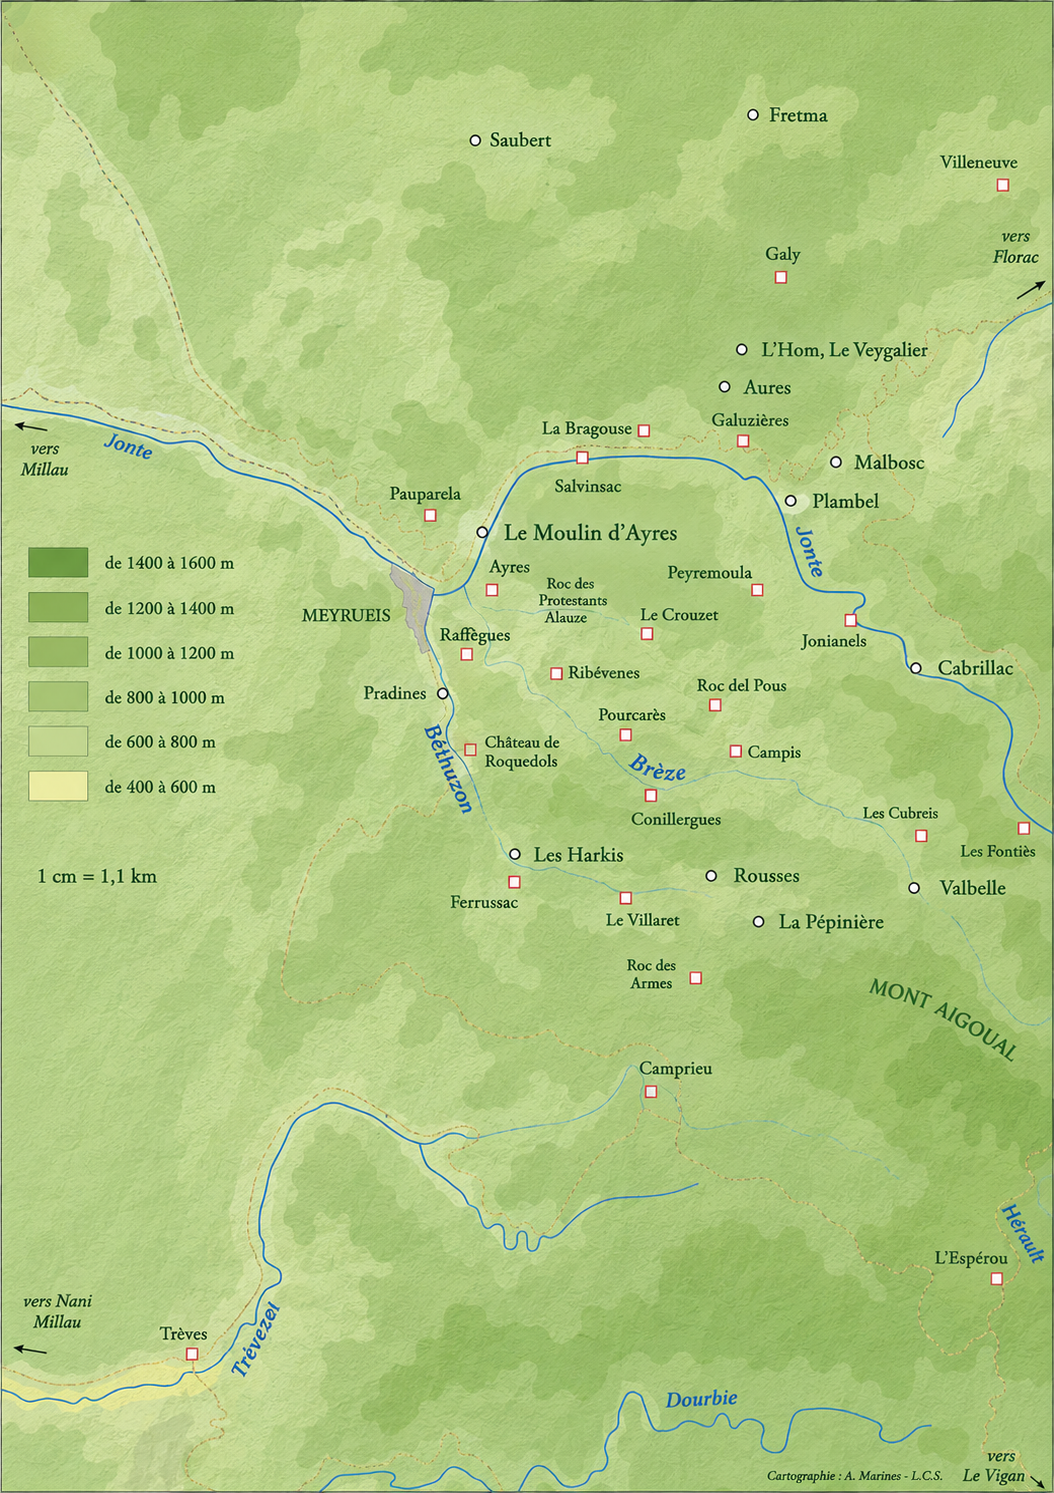
\includegraphics[width=0.85\paperwidth,height=0.85\paperheight,keepaspectratio]{imgs/004.png}


\clearpage

% La première page numérotée du document original est la page 1.
\setcounter{page}{1}

\input{pages/005-Avant-propos}
\clearpage

\input{pages/006-Lettre-Henri-Belon}
\clearpage

\input{pages/007-trois-figures}
\clearpage

% Page 019 — page imprimée 15
% Une épidémie à Meyrueis en 1768
% Reconstruction éditoriale en LaTeX.

{\fontsize{10.25}{12.1}\selectfont

\sectiondate{Une épidémie à Meyrueis}{1768}


\begin{center}
\fbox{%
\begin{minipage}{0.91\textwidth}
\itshape
Ce compte rendu d’inspection médicale à Meyrueis et dans les environs a été rédigé en 1768, vingt ans avant la révolution. On peut le consulter au Service du Patrimoine de la Médiathèque de Montpellier sous la cote 19.180.

\vspace{0.35em}

Il m’a vivement intéressé pour trois raisons :

\vspace{0.15em}

1/ \quad La description assez précise de cette épidémie dénommée « peste blanche » conséquence du manque d’hygiène, de la pauvreté et d’une nourriture insuffisante et souvent avariée.

\vspace{0.15em}

2/ \quad L’évocation de la vie quotidienne des paysans de Meyrueis et des vallées des environs à la suite de mauvaises récoltes dues à des sécheresses persistante et à des hivers rigoureux. Les maisons ne sont que des masures sans aération où « l’on meurt de froid ou de chaud », la promiscuité est générale, excellent terreau pour la tuberculose et toutes les maladies infectieuses.

\vspace{0.15em}

3/ \quad Le style et les tournures surannées de ces lignes.

\vspace{0.15em}

Ce mémoire complète donc ce que l’on peut savoir de la vie de nos aïeux à Meyrueis mais aussi à Carnac près de Rousses où la famille Couderc résidait alors.
\end{minipage}}
\end{center}

\vspace{5mm}

\begin{center}
{\fontsize{18}{20}\selectfont\bfseries MEMOIRE\par}
\vspace{0.55em}
{\bfseries
sur la maladie épidémique\\
qui a régné à Meyrueis et ses environs
}
\vspace{0.15em}

Présenté à Monsieur de Saint Priest\\
Le 3 Septembre 1768

\vspace{0.35em}

{\bfseries Par Tandon, Docteur en Médecine\par}
Imprimé par Auguste François Rochard, Place du petit Scel\\
Montpellier 1769
\end{center}

\vspace{0.55em}

C’est une maladie qui a régné assez longtemps dans une partie très considérable des Hautes Cévennes, manifestée par des fièvres intermittentes d’un très mauvais caractère. Elles ont d’abord sévi à St Jean de Védas, la Verune, Fabrègues, Gigean, Loupian, Cournon venant des exhalaisons des étangs par fortes chaleurs et de mauvaises récoltes. Le plus grand nombre des habitants est obligé de se nourrir d’\textit{azéroles}\footnote{Fruit de l’azérolier, jaune ou rouge, ressemblant à une petite pomme}, de mûres de haies, de figues et de raisins qui n’étaient pas mûrs et de petites carpes, muges, anguilles et loups.

Puis l’épidémie s’est répandue sur Marsillargue, Clermont, Lodève, Mèze et enfin les Hautes Cévennes.

\vspace{0.3em}

}

{\fontsize{10.25}{12.1}\selectfont
La maladie épidémique qui règne depuis environ cinq mois, parmi les gens de la campagne à Meyrueis et ses environs, Lanuéjols, Montjardin, Serviglières et quelques autres lieux moins considérables, est une fièvre, maligne, bilieuse, qui, à ce qu’on affirme, a fait de grands ravages à Séverac en Rouergue et a parcouru le Vallon du Tarn. Cette maladie prélude pendant plusieurs jours des malaises, des lassitudes, des pesanteurs d’estomac, le dégoût et le cours de ventre bilieux... la langue auparavant rouge, sèche, se racornit, se fend en différents sens et se retire dans le fond de la bouche, ou se couvre d’une croûte noirâtre et raboteuse qui s’étend sur les gencives et les lèvres qu’elle fait paraître brûlées et dans cet état ils ne peuvent ni parler ni avaler à moins qu’on ait l’attention d’humecter souvent ces parties.

\begin{itemize}
\item Il est très douteux qu’on ait vus des bubons.
\item Le terme le plus ordinaire est du quatorzième ou quinzième jour, parfois 22 ou 23.
\item Les enfants en ont tous réchappé mais à Lanuéjols il y a eu 45 morts.
\end{itemize}

\medskip
\textit{Quelles sont les causes les plus apparentes de cette épidémie ?}


« L’excessive misère qui règne depuis longtemps parmi les habitants de ces montagnes. La mauvaise nourriture et la malpropreté qui en sont inséparables, les alternatives de froid et de chaud, les orages mais surtout les brouillards qu’ils y ont presque continuellement essuyés. Une longue suite de mauvaises récoltes a rendu cette misère si sensible qu’à ne considérer que l’état actuel de ces infortunés, on ne saurait se persuader qu’ils aient jamais pu être les pères nourriciers de la plus grande partie des Cévennes...

... relégués dans le fond des vallons, tous couverts de haillons et ayant à peine une chemise de rechange, ils y habitent de misérables chaumières placées sur le bord de quelque torrent et entourées de fumiers de buis qui exhalent une odeur des plus insupportable....

... obligé de pénétrer dans ces chaumières on est tout étonné de voir que l’air intérieur de ces réduits obscurs et malsains y est à grand peine renouvelé par l’ouverture étroite d’une ample cheminée, d’une porte écrasée et d’une fente qui tient lieu de fenêtre pratiquée sur l’un des côtés de cette porte et de n’y trouver que quelques mauvaises planches mal assurées dans le mur, dont ils n’ont maintenant que faire, mais qui, autrefois, leur servaient à ranger leurs denrées...

... on y distingue également un vieux coffre où ils tiennent leur peu de provision, et une vaste caisse carrée remplie de feuilles de frêne couverte de quelques lambeaux de grosse toile et d’une mauvaise couverture, qui leur sert lieu de grabat sur lequel le vieillard décrépit et l’enfant nouvellement né, la fille et le garçon, le sain et le malade, le mourant et le mort sont souvent confondus....

Leur nourriture ordinaire est de l’orge la plus grossière dont ils font un peu de pain, ou qu’ils font cuire avec le lard le plus rance qui leur sert ensuite de pitance. On les a vus, en dernier lieu, faire le bouillon ou la soupe pour leurs malades avec le vieux oing\footnote{Vieille graisse de porc fondue servant à graisser un mécanisme.}.

Les autres aliments dont ils usent sont les aulx, les oignons et, en hiver, quelques pommes de terre, des raves, les plus mauvais légumes et des fromages encore plus mauvais.

Aussi en est-il mort un très grand nombre.

}

{\fontsize{10.2}{12.0}\selectfont

Dans des temps plus heureux on les a vus se nourrir d’assez bon pain de froment, de bons légumes, d’un peu de viande fraîche, de cochon salé, de harengs et de morue, de châtaignes et d’assez bon fromage et se procurer une quantité suffisante de linge pour se tenir propres, et se coucher sur la paille qu’ils avaient soin de renouveler assez souvent…

Cette maladie, quoique très dangereuse par elle-même n’eut point eu de suites si fâcheuses si, par une fatalité dont on a peu d’exemples, la plupart des malades n’eussent été presque entièrement privés de secours :

Mr Auzilion, chirurgien de Meyrueis, qu’on a eu le malheur de perdre vers le milieu de cette épidémie a été pendant longtemps le seul qui les ait visités et leur ait administré des remèdes. Mais malgré sa bonne volonté et une très grande activité il lui était impossible de les visiter tous et aussi souvent qu’il eut fallu, vu leur nombre, leur éloignement et leur dispersion…

Depuis sa mort jusqu’à mon arrivée, aucun d’eux n’avait été vu que par M. Fignel curé de Lanuéjols.

Aussi en est-il mort un très grand nombre qui n’avaient pris pour tout remède que du suc d’oignon blanc, mêlé avec de la mauvaise huile ou de la suie détrempée dans du vinaigre ; remède réputé souverain parmi eux pour les maladies de la nature de celle-ci, qu’ils qualifiaient de peste blanche…

\medskip
\textit{Pour arrêter les progrès de cette maladie :}

\textbf{1/} On exhortera tous les habitants de la campagne à se tenir aussi proprement qu’il serait possible en leur faisant sentir toute la nécessité d’emporter à des distances assez éloignées le fumier qui entoure leurs chaumières, de nettoyer le dedans de renouveler souvent leurs grabats, de changer de linge et de ne s’exposer au grand air que lorsque les brouillards seront entièrement dissipés.

\textbf{2/} Il sera journellement distribué aux nécessiteux, en danger de tomber malades, à raison de leur détresse, un peu de viande fraîche, du cochon salé, du pain second, quelques légumes et même s’il était possible, un peu de vin et une certaine quantité de linge de rechange.

\textbf{3/} Les médecins feront tous les jours la visite des malades et auront, chemin faisant, la plus grande attention sur ceux qui seraient menacés de la maladie, pour les en garantir, s’il était possible, en leur prescrivant la diète, les boissons les émétique, les purgatifs et les stomachiques convenables.

\textbf{4/} Vu l’état de dépérissement et de faiblesse dans lequel se trouvent la plupart des malades ils soutiendront leurs forces par de bons bouillons, de légers cordiaux et des tisanes légèrement incisives… Ils seront très réservés sur les saignées, les émétique et les purgatifs… En espérant que les approches d’une saison plus tempérée contribuera à terminer bientôt cette fâcheuse maladie.

\vspace{0mm}

\begin{tcolorbox}[
  colback=white,
  colframe=black,
  boxrule=0.7pt,
  arc=0pt,
  left=6pt,right=6pt,top=5pt,bottom=5pt
]
\textbf{On peut penser, sans grand risque d’erreur, que la misère extrême du pays et particulièrement des vallées comme du village de Lanuéjols, autrefois protestant, était une conséquence des persécutions et des dragonnades qui, après le brûlement des Cévennes de 1703, continuèrent tout au long du 18\ieme{} siècle.}
\end{tcolorbox}

}



\clearpage

\input{pages/009-foires}
\clearpage

\input{pages/010-société-populaire}
\clearpage

% Page 024 — page imprimée 20
% Protestants et Catholiques face à la Révolution à Meyrueis et dans les Cévennes


{\fontsize{10.15}{11.65}\selectfont

\sectiondate{Protestants et Catholiques face à la Révolution}{1789-1795}

\begin{center}
{\Large\bfseries Protestants et Catholiques face à la Révolution\\
à Meyrueis et dans les Cévennes}

\vspace{1.0em}

{\bfseries 1789 -- 1793}
\end{center}

\vspace{0.55em}

Meyrueis, comme toutes les Cévennes méridionales, s’engage dans la Révolution avec ardeur.
La majorité de la population ayant abjuré du bout des lèvres, était restée attachée à la Réforme et avait accueilli avec joie l’Edit de Tolérance de 1797 qui leur permettait de retrouver un état civil pour leurs familles.
Avec la Révolution les protestants étaient désormais des citoyens à part entière. Les campagnes cévenoles envoyèrent donc à l’Assemblée Constituante une majorité de « patriotes ».

Mais l’année 1789 avait été une mauvaise année : les récoltes médiocres après un hiver glacial et les difficultés économiques de toutes sortes provoquèrent des troubles. Uns grande peur touche aussi les communautés protestantes qui ont tout à craindre d’une réaction catholique.
Les persécutions et les dragonnades sont dans toutes les mémoires.
Les différences confessionnelles imprègnent celles des comportements. Le choc décisif est la question religieuse.

\medskip

\textbf{La réaction catholique}

\vspace{0.45em}

L’Assemblée Constituante vota, en effet, la vente des biens nationaux et la Constitution Civile du Clergé exige de tous les prêtres un serment de fidélité à la Constitution. Dès lors les prêtres se divisèrent en « constitutionnels », ou « réfractaires » nombreux dans le nord de la Lozère.
Le pape Pie VI condamnant cette constitution, il y eut schisme dans l’église catholique : la plupart des prêtres réfractaires prennent le parti de la contre-révolution : certains émigrèrent d’autres furent massacrés pendant la Terreur (1792-1794).

Comme les chouans en Vendée, le nord de la Lozère, à partir des Gorges du Tarn se dressa contre la République laïque et anticléricale. Des bandes se formèrent pour lutter contre les « patriotes ». Une véritable petite armée était disponible pour des coups de main ou de véritables batailles, dirigées par un chef noble, originaire de Nasbinals, Marc-Antoine Charrier, député du Gévaudan.

Des « républicains » furent tués et la situation devint si grave que la République envoya des troupes pour stopper « les rebelles ». Beaucoup furent arrêtés dont les principaux chefs.
Charrier s’était aménagé une « cache souterraine » dans sa maison de Nasbinals. Mais il fut vendu et il sera fusillé à Rodez. C’est ainsi que dans la région la loi prévoyait « la mort pour les chefs et la clémence pour leurs troupes ». Mais le tribunal de Mende passa outre, après l’arrestation d’un groupe de 40 paysans de la Malène. Trente-
sept furent exécutés à Florac. Trois d’entre eux avaient-ils réussi à s’échapper ? Une plaque rappelle leur mort dans l’église de la Malène.\footnote{\fontsize{8.0}{9.25}\selectfont
\textit{« Jean-Baptiste Fages de la Malène, frère d’un rebelle guillotiné à Florac en Juin 1793, est le chef de la première bande organisée.
Ses hommes se retrouvent lors d’expéditions punitives contre « les patriotes » et le reste du temps réintègrent leurs foyers et cultivent leurs champs.
Le lieutenant de Fages est un jeune déserteur des armées républicaines, natif de Hures, sur le Causse Méjean connu sous le sobriquet de Ferratou. Tous deux sont arrêtés en Janvier 1794. Fages périt à l’échafaud alors que Ferratou parvient à s’échapper. A la tête de sa bande il fut repris un des jours suivant et fusillé à Meyrueis ».}
}
}

\vspace{0.25em}


% Page 025 — page imprimée 21
% Protestants et Catholiques face à la Révolution à Meyrueis et dans les Cévennes


{\fontsize{10.05}{11.45}\selectfont

\textbf{L’engagement protestant}

\vspace{0.35em}

Il ne fait pas de doute que les protestants de Meyrueis ont accueilli favorablement la
Révolution. Nous ne disposons pas, à ma connaissance, de beaucoup de documents en
donnant la preuve si ce n’est un mémoire de Antoine Avesque (1771-1834) que l’on trouve
dans un registre de son fils, Pierre Calixte Avesque, notaire. Il gérait le domaine de Drigas et
avait affermé également, avec trois coreligionnaires (Bosc, Belon et Avesque), le domaine de
Saubert. En voici les premiers paragraphes transmis par Me. Pottier, notaire à Meyrueis, qui a
rajouté la ponctuation, et corrigé l’orthographe :

\begin{center}
\textbf{Au nom de Dieu soit fait Amen}
\end{center}

Livre de mémoire où on pourra trouver note des affaires majeures et essentielles que j’ai pu traiter, y puiser
bien des renseignements, certains faits et sur diverses affaires…

\begin{enumerate}[label=\arabic*., leftmargin=2.0em, itemsep=0.55em, topsep=0.25em]
\item
La Révolution commença en l’année 1789. Louis XVI ayant convoqué les Etats Généraux, ils finirent
par se rendre maître du pouvoir souverain et par lui faire porter la tête à l’échafaud ainsi que de
perdre toute la famille royale. Quasi toute la noblesse française émigra aux époques de 1791-1792.
Tous les souverains d’Europe se liguèrent contre la France il y eut des guerres terribles, les Français
restèrent toujours vainqueurs, malgré la faiblesse de nos gouvernants, malgré les guerres civiles qui régnaient
dans plusieurs point de France comme à la Vendée, à Lyon, en Lozère, en Ardèche etc. et malgré la trahison de
plusieurs généraux.

Les prêtres qui n’avaient pas voulu prêter le serment de fidélité à l’Etat furent fortement persécutés. On en fit
périr plusieurs. Par la suite les ministres (les pasteurs) le furent aussi mais d’une manière moins forte.
Dans ce temps on abattit beaucoup de cloches et de clochers, le peuple se porta à des excès de fureur en brûlant
les châteaux et les maisons de certaines personnes qu’on appelait suspects. Enfin la France était dans le plus
grand désordre, l’Histoire en fournira les détails.

\item
A l’époque, au mois de Juillet 1790 je fus député avec M. Ricard par le district de Meyrueis pour aller à Paris à la
grande fédération du 14 Juillet…

\begin{quote}
…A l’époque du 10 Aout 1792, nous partîmes environ \textbf{quatre vingt sept jeunes gens de Meyrueis ville et
Meyrueis campagne}, tous de bonne volonté pour la défense de notre patrie. Nous formâmes notre bataillon à
Mende. Je fus nommé capitaine. J’ai fait quatre campagnes dans les Alpes… Notre bataillon était le premier de
la Lozère.

\textit{De ces 87 jeunes conscrits combien ont échappé à la mort ?}
\end{quote}
\end{enumerate}

\vspace{0.15em}

Ainsi la 3\ieme compagnie du 1\ier Bataillon de l’armée des Alpes était composée
exclusivement de Meyrueisiens. Elle avait à sa tête trois tout jeunes officiers :

\begin{itemize}[leftmargin=1.8em, itemsep=0.18em, topsep=0.2em]
\item Antoine Avesque, 24 ans, capitaine
\item Pellet, lieutenant
\item Mezin, 1,69m, blessé d’un coup de feu à l’affaire du 28 Messidor an IV sous Mantoue :
la balle lui a traversé la poitrine. A la bataille de Wagram il reçoit deux coups de feu :
l’un lui traverse la jambe droite l’autre lui emporte le bout du nez. Il reçoit la Légion
d’Honneur pour la conduite distinguée qu’il a tenue à Porto-Vecchio en Corse. Il
meurt, chef de bataillon à l’hôpital d’Anvers après 21 ans de service.
\end{itemize}

On trouve encore deux autres meyrueisiens au 3\ieme bataillon

Jean Cambon, 18 ans, Lieutenant et François Vivens, 24 ans, sous-lieutenant qui se
retire à Meyrueis en l’an IV après quatre ans de service. Il est considéré comme
déserteur.

}


\clearpage

% Page 026 — page imprimée 22
% Contenu seul : le préambule et la pagination sont gérés par meyrueis.tex

\sectiondate{Histoire de Samuel François}{1789-1795}

\begin{center}

\vspace{0.45em}

{\large\bfseries Pasteur de Meyrueis, nommé Administrateur\\
du Département de la Lozère}

\vspace{0.45em}

{\small\bfseries\itshape
D’après les comptes-rendus de la Société Populaire de Meyrueis\\
Archives Gévaudanaises : 1913. JB Belon P. 293 à 316}
\end{center}

\vspace{0.7em}

A cette époque Meyrueis avait bénéficié du ministère pastoral de Samuel François.
Écœuré sans doute, par les excès de la Révolution il avait été nommé chef du parti Girondin de
Lozère. Il soutenait un certain fédéralisme au point qu’il fut jeté en prison à Mende. Il réussit
à s’évader et les Montagnards se jetèrent à sa poursuite.

C’est ainsi qu’arriva à Meyrueis, le 6 germinal (27 mars 1794), le Montagnard Chateauneuf-
Randon qui, prenant la parole « avance, dit-il, avec regret, qu’il est convaincu qu’il existe
dans la commune des citoyens instruits du lieu de la retraite de Samuel François ; il démontre
avec fermeté le crime de la récelation (sic) et propose de faire une adresse au peuple pour
l’éclairer de son devoir. »

A ces mots la Société par un mouvement spontané se lève et jure de révéler tout ce qu’elle
pourra découvrir de relatif à la retraite de « cet homme pervers qui a tenté, mais en vain,
d’avilir la représentation nationale et d’égarer le peuple sur ses véritables intérêts ».

Samuel François reste introuvable ; Chateauneuf-Randon décide alors de faire incarcérer sa
femme, mère de plusieurs enfants. Son sort émeut quelques anciens paroissiens de son mari à
Meyrueis, et lors d’une séance du Comité, le 24 vendémiaire an III (16 Octobre 1794) l’un
d’entre eux prend la parole et s’exprime en ces termes :

\begin{quote}
\itshape
« Citoyens, je viens intéresser votre justice, votre humanité en faveur de la citoyenne
François, dont le civisme, depuis 1789, ne s’est jamais démenti. Vous avez été les témoins de
sa conduite pendant la Révolution. Vous connaissez ses malheurs et la pureté de ses
intentions ; vous êtes instruits des motifs qui l’ont privée de sa liberté.

Vous savez qu’elle est en arrestation par ordre du représentant du peuple Châteauneuf-
Randon, depuis plus de six mois. Vous n’ignorez pas que l’évasion de son mari fut la seule
cause de cette mesure de sûreté générale. Vous savez encore que cette citoyenne a une
famille qui ne vit que de son travail et que son absence a réduite à la dernière misère. Ces
motifs de justice et d’humanité basent une réclamation qui tend à ce que la Société se
prononce en faveur d’une citoyenne intéressante par ses malheurs et son civisme, et qu’elle
sollicite sa mise en liberté auprès du comité de Sûreté Générale de la Convention. Plusieurs
membres parlent de la citoyenne François et tous manifestent le même sentiment à son égard.

L’assemblée arrête à l’unanimité que le comité de Sûreté Générale de la Convention sera
invité d’ordonner la mise en liberté de la citoyenne Samuel François de Meyrueis, détenue
dans la maison de réclusion de Mende par ordre du représentant du peuple Châteauneuf-
Randon. »
\end{quote}

% Page 027 — page imprimée 23
% Contenu seul : le préambule et la pagination sont gérés par meyrueis.tex

\textbf{Il avait donc fallu 6 mois pour qu’un membre du Comité Populaire se soucie du sort de
la femme du pasteur Samuel François, et ose, suivi par tous les membres du Comité
Populaire de Meyrueis, se dresser contre la mesure unique prise par Châteauneuf-
Randon. !!!}

Quelques mois plus tard, les poursuites contre Samuel François sont levées. Il peut reparaître
en plein jour, et regagne Meyrueis, sa famille et les séances de la Société Populaire. Voilà
comment est relaté son retour (séance du 21 ventôse An III (11 mars 1795).

\begin{quote}
\itshape
«\ldots\ Un sujet intéressant devait fixer dans cette séance l’attention et l’attendrissement de
chaque citoyen : c’était le récit de la persécution affreuse à laquelle a été en butte toute une
année, l’honnête citoyen dont tout le crime était d’avoir osé défendre les droits du peuple. Il a
demandé d’être réintégré dans la Société ; il a même produit des preuves de son civisme
reconnu pendant sa fuite ; mais l’assemblée assez pénétrée depuis longtemps des vertus
énergiques du citoyen Samuel François, l’a admis comme par l’acclamation et l’accolade
fraternelle qu’il a reçue des membres du bureau, lui est un sûr garant de la joie que ressentait
la Société du recouvrement d’un membre, dont l’absence n’avait pu, que se faire sentir
vivement dans son sein et dans l’administration du Département, dont il était membre. »
\end{quote}

\textbf{En mars 1794 personne n’avait osé, au moins en public, prendre la défense de Samuel
François alors qu’il venait de s’évader : ce n’était qu’un scélérat, mais un an plus tard,
en Mars 1795, les membres de la Société se jettent à son cou comme si de rien n’était.}

Il est vrai que \textbf{Châteauneuf-Randon} (\textit{de son vrai nom Alexandre Paul Guérin du
Tournel, marquis de Joyeuse, Comte de Châteauneuf-Randon}) et ses méthodes violentes
ne sévissait plus en Lozère. (Il lui fallait bien faire la preuve, lui, l’aristocrate, qu’il était un
vrai montagnard -- révolutionnaire). Il avait été \textbf{nommé auprès de l’armée des Pyrénées}.

\vfill

\begin{center}
\small
Extraits des comptes-rendus de la Société Populaire de Meyrueis,\\
édités par la Société d’Agriculture, Industrie, Sciences et\\
Arts de la Lozère, 1913. Archives Gévaudanaises\\
Mars 2006
\end{center}

\clearpage

\input{pages/013-Meyrueis}
\clearpage

\input{pages/014-fabrique-pointes}
\clearpage

\sectiondate{Mémoire sur la ville de Meyrueis}{1881}

« ...C’est une contrée intéressante : la cinquième ville du Diocèse Elle est habitée par une
noblesse et une bourgeoisie nombreuse. On y compte en ce moment douze Chevaliers de St.
Louis et beaucoup d’autres militaires au service du Roi ; beaucoup de bourgeois vivant
noblement, plusieurs avocats ou gradués ; quatre offices de notaire, ses fabriques d’étoffe de
laine de son cru qui partent presque toutes pour l’étranger ne pouvant être servies que par ses
habitants.

Le commerce qui s’y fait des plus beaux mulets du Royaume et des meilleurs moutons la rend
pour ainsi dire, l’entrepôt de la Provence, des provinces voisines et même de l’Espagne.
C’est la mère nourrice des Cévennes par le blé qu’elle leur fournit.
...Il faudrait supprimer toutes les justices bannerettes... que les places de judicature ne
fussent plus vénales, que ce fut le mérite seul qui put y appeler et que le tarif le plus exact
réglât tous les droits ».

\begin{quote}
\itshape
Mémoire sur la ville de Meyrueis, (Annuaire de la Lozère 1881) ainsi que la prise du Malzieu
le 17 Novembre 1573 Pages 3 et ss. \quad Notices rédigées par Fernand André, Archiviste.
\end{quote}

\clearpage

% Page 030 — page imprimée 26
% Contenu seul : le préambule et la pagination sont gérés par meyrueis.tex

\sectiondate{Nous avons remnoté la vallée de schiste bleu...}{1884-1894}


\vspace{3.0em}

Sur la place du village : une fontaine, ronde, lisse, usée ; un arrosoir s’emplit pendant que
l’autre attend.

Derrière la fontaine, à deux pas coule la rivière : elle partage le village en deux, mais sept
ponts relient les deux moitiés.

A l’angle de la place, la Tour de l’Horloge sonne les heures, sourdes de neige ou vibrantes de
soleil selon l’humeur du temps.

Et la vie s’organise autour : le porche des boulangers et des bouchers, le marché dallé et
couvert, les platanes, le café de l’Union, l’Etoile du midi et le pont des Mensonges.

D’un côté les maisons s’adossent au Causse, presque à pic, et de l’autre, elles remontent dans
les vallées, vers l’Aigoual. Pour se situer il faut toujours lever les yeux : là haut en bordure du
ciel, c’est le Causse clair avec sa couronne de pierre, là-bas vers un horizon plus lointain, c’est
l’Aigoual plus sombre avec ses forêts.

Enfants, nous allions à pied, nous remontions les vallées jusqu’à la forêt, au château, au
moulin, mais jamais nous n’atteignions ni l’Aigoual ni le Causse ; ils étaient trop loin, trop
hauts.

Les gens de là-haut descendaient au village acheter, vendre, parler, prier, danser ; ils
amenaient du bois et des fromages, des raves et des grives, leur allure était différente, alors on
imaginait...

Quand nos parents parlaient du temps c’est l’Aigoual qu’on regardait, c’est lui qui envoyait
les nuages de la pluie : \textit{« S’il tonne vers l’Aigoual, prends tes bœufs et rentre à l’oustal.\footnote{Se trona vèrs l'Aigoual, pren tos buòus e torna a l'ostal} »}
Quand la pluie ne venait plus et que la sécheresse s’installait, c’est le Causse qui souffrait ; les
brebis dévalaient, en faisant rouler les pierres blanches, vers notre maigre rivière, pour boire,
boire, boire...

En Septembre, parfois, l’eau déboulait en trombe de l’Aigoual. On disait \textit{« L’eau est
grosse »} ; les troncs d’arbres passaient sous les ponts, tout le village était dehors, les gosses
couraient d’un parapet à l’autre...

Quand la neige, soufflée par le vent, balayait le plateau et se tassait dans les creux, c’est le
Causse nu, sans repères, sans abris, qui devenait l’enfer, la peur de mourir seul, perdu, gelé.

Mais chaque année arrivent les myrtilles et les mousserons, le buis se redore, le chardon
s’épanouit, les brebis appellent leurs agneaux et les perdrix se promènent « en compagnie ».

Au carrefour de nos vallées étroites, toute cette vie se mêle et se confond. Les deux génies de
la montagne, l’un de granit, l’autre de calcaire, nous observent, nous inquiètent et nous
protègent.

Ils détiennent le pouvoir de l’eau ; haut placés, ils captent les nuages et chacun d’entre nous
les renvoie à sa façon : le Causse boit l’eau goulûment et la rejette au bas de la falaise, tandis
que l’Aigoual la laisse couler à l’air libre sur des kilomètres, tout le long des vallées.

% Page 031 — page imprimée 27
% Contenu seul : le préambule et la pagination sont gérés par meyrueis.tex

Au carrefour de nos vallées étroites toute cette vie se mêle et se confond, ces deux génies de
la montagne, l’un de granit, l’autre de calcaire, nous observent, nous inquiètent et nous
protègent.

Ils détiennent le pouvoir de l’eau ; haut placés, ils captent les nuages et chacun d’entre nous
les renvoie à sa façon : le Causse boit l’eau goulûment et la rejette au bas de la falaise, tandis
que l’Aigoual la laisse couler à l’air libre sur des kilomètres, tout le long des vallées.

Ici, l’eau joue un grand rôle : avalée par les avens, calcifiée dans les grottes, creusant des
gorges célèbres. Pour nous, cela est naturel, nous l’avons toujours vu.

Paradoxalement, nos émotions les plus fortes nous les avons ressenties avec les sources, ces
jaillissements spontanés, imprévus, connus des seuls initiés.

Des sources il y en a partout dans les vallées : celle du Pied Pointu qui sort à deux pas du ciel,
est directement branchée sur les nuages ; les bergers ont mis quatre pierres pour la retenir un
peu. Seuls quelques myosotis et une végétation insolite la trahissent ; elle est là, silencieuse,
moqueuse, elle passe directement du ciel au ventre de la terre.

Il y a la « gourguette » qui jaillit au bord de la route pour le passant, « la fontaine de
Paul » qui sort presque dans la rivière, celle du « serre » bien placée pour les moissonneurs et
le troupeau et que l’on surveille de près de peur de la perdre...

Et puis un jour, nous avons remonté la vallée de schiste bleu jusqu’à l’horizon ouvert, jusqu’à
la source de la rivière. Toute une journée nous avons arpenté forêts et pâturages.

Et, là-haut, nous avons connu le granit, ces grosses boules belles comme des bijoux,
imbriquées en jeu de construction monumentaux, piédestal des rapaces.

Nous avons rencontré le troupeau transhumant. Il enroulait et déroulait son chemin de laine et
le mouton disparaissait dans le troupeau vivant.

Le soir nous avons couché au sommet pour assister au lever du soleil car ici, l’arrivée du jour
est un moment rare, mais le soleil, dans les brumes, n’est apparu qu’à dix heures, frileux et
moqueur....

Ce jour-là, nous avions déchiré un petit bout du mystère de l’Aigoual.

\begin{flushright}
Janine BRAGER
\end{flushright}

\begin{flushright}
Extraits de « Cévennes et Grands Causses »\\
d’Alain Gas Presses du Languedoc p.13-14
\end{flushright}

\vspace{0.6em}

\begin{center}
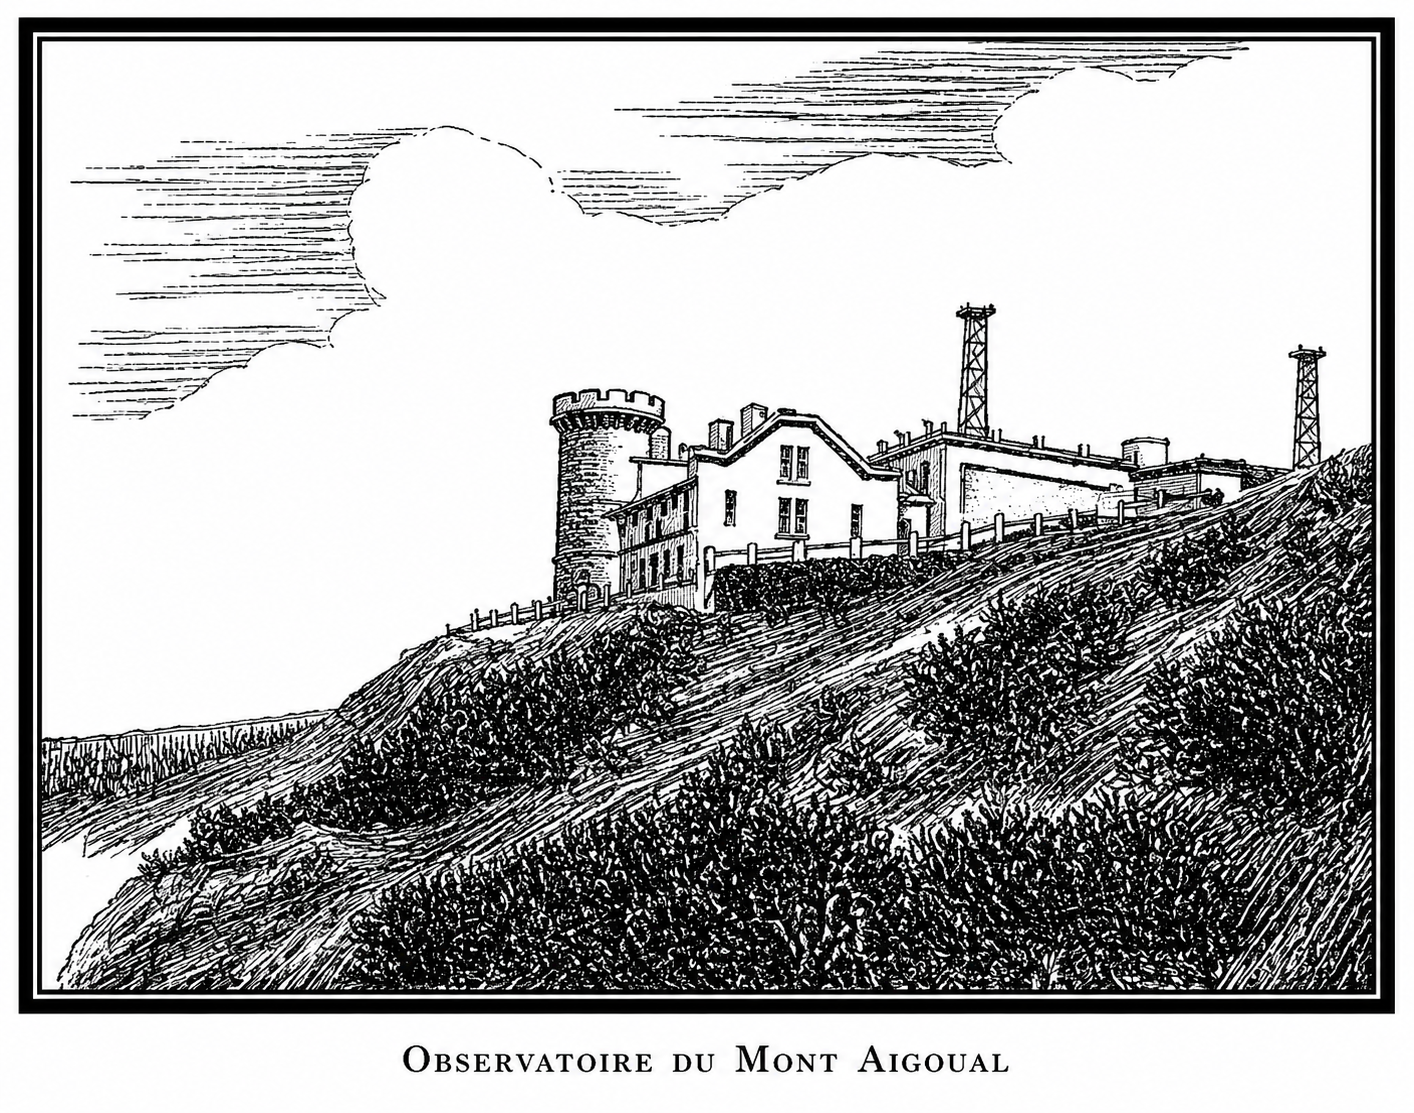
\includegraphics[width=\textwidth]{imgs/031.png}
\end{center}

\clearpage

\input{pages/017-chapeliers}
\clearpage

% Page 036 — page imprimée 32
% Contenu seul : le préambule et la pagination sont gérés par meyrueis.tex


\sectiondate{La  grotte de « La Douce »}{1920}


\vspace{1.5em}

\textit{Son entrée, au dessus du Ferradou, sur le vieux chemin montant au rocher du Château, servit
longtemps de bergerie pour quelques brebis. C’est seulement en 1920 que Frank Loupiac et
son jeune cousin, Daniel Couderc\footnote{Daniel Couderc 1908-1997, fils de Léon Couderc et Madeleine de Felice, cousin germain de Frank Loupiac}, découvrirent, les premiers, le début du réseau de la
Douce\footnote{La Douce signifie « la Source ». cf André Fages : « La quête de l’eau » 2004 «
Los Adrelhans ». Le hameau « des Douze » tire aussi son nom de cette étymologie.} qu’on appelle maintenant grotte de la Porte. Philippe Chambon en est propriétaire et dispose des clefs.}

\textit{Voici le récit de cette première « exploration » tel qu’elle nous a été contée par Daniel
Couderc et enregistrée au Moulin d’Ayres au cours de l’été 1981.}

\vspace{1em}

« Comme la plupart des enfants j’ai longtemps aimé l’obscurité. Quoi de plus rassurant
lorsqu’on a deux ans de se blottir sous les couvertures tout contre la chaleur maternelle, la
conscience épanouie par de vagues et heureuses réminiscences. Plus tard vers 4 à 6
ans l’aventure se complique : elle consiste à se frayer soi-même un chemin vers la lumière,
vers le bout du lit étroitement bordé « à la française » : plus tu avances et moins il y a de
place. La tête sert de butoir, elle écarte et soulève les draps pour trouver un peu d’air, il fait
chaud, tu étouffes... Mais voilà que ton bras s’est glissé au dehors, il te tire vers la fraîcheur...
Encore un effort et tu débouches en riant tout près de tes parents dans la chambre ensoleillée
par une matinée de printemps. C’est plus tard que pour beaucoup, l’obscurité se peuple d’êtres
malfaisants : fantômes, vampires, araignées ou reptiles venus de légendes racontées par des
adultes irresponsables !!!

Il est possible que ces « histoires » aussi vieilles que l’humanité ne soient elles mêmes que le
reflet d’une crainte ancestrale venue des temps où l’obscurité était en effet pleine de pièges.
Mais c’est là une autre question...
Heureusement, et grâce à des parents éclairés, notre imagination fut préservée de ces craintes
irraisonnées, de même que celle de mon cousin Frank.

Bien qu’il soit mon aîné de 3 ans, nous nous entendions à merveille lorsque je le retrouvais à
chacun de mes séjours à Meyrueis. Il me montrait la rivière ou plutôt les trois rivières qui se
rencontrent à Meyrueis.
Pêcheur émérite il en connaissait tous les « gouffres », et lorsqu’il partait en expédition,
parfois pour toute la journée, il ne revenait jamais bredouille. Mais il aimait aussi les trous, les
grottes, les avens qui abondent dans la région et là, je le suivais avec passion.

En cette année 1920, j’avais 12 ans, lui 15 nous avions décidé de réaliser un projet qui nous
tentait depuis longtemps : nous voulions explorer la grotte de la Douce. La Douce n’est pas
une rivière, même pas un ruisseau, c’est seulement une cascade parfois impétueuse qui se
manifeste après une période de mauvais temps et de pluies abondantes. Elle jaillit du rocher et
tombe presque directement dans la Jonte juste derrière notre maison. Le trou d’où elle sort
parfaitement sec en été est trop étroit pour être remonté au-delà d’une dizaine de mètres mais
son débit lorsqu’elle fonctionne montre qu’elle est le déversoir de tout un réseau de galeries
souterraines s’étendant sous le Causse. Comment atteindre ce réseau ?»

Une ouverture triangulaire située très haut dans le rocher qui dominait notre vue du Ferradou
aurait pu être un accès. Mais après une escalade hasardeuse, accomplie au printemps avec
corde et pitons, Frank s’était rendu compte que ce trou ne permettait aucune approche
intéressante…

Restait la « Bergerie ». C’était une caverne qui s’ouvrait dans un petit champ à une centaine
de mètres au dessus de notre maison. Elle était fermée par une porte de bois à laquelle on
accédait par un chemin profond creusé entre le champ et la falaise. Le propriétaire s’appelait
« Luquet ». Il nous prêta la clef en riant : \textit{« Vous ne trouverez rien dans ma caverne, nous dit-
il, à part des crottes de brebis !… On pouvait bien y loger 200 bêtes autrefois, moi je n’ai pas
le temps de « tenir » le troupeau. »} En arrivant nous trouvâmes que la porte n’avait plus de
serrure. Des vagabonds s’étaient peut-être abrités là pendant l’hiver…

La caverne avait l’aspect d’une longue salle rectangulaire d’environ 20m sur 5, recouverte par
un rocher sans fissure. Nous marchions sur une couche élastique de très anciennes crottes de
mouton, parfaitement sèches et sans odeur. Au fond s’élevait une masse calcaire, un peu
comme un autel dans le chœur d’une église.
On pouvait en faire le tour par une galerie relativement étroite dans laquelle s’ouvraient
quelques trous à différentes hauteurs. L’un d’eux, au ras du sol, était plus profond que les
autres. C’était un véritable boyau dans lequel nous nous \textit{engageâmes d’abord en courbant le dos,
puis à genoux, enfin en rampant à mesure que la voûte s’abaissait au dessus de nous.} Le sol
était meuble, friable : un limon desséché depuis des siècles !

Frank était devant moi avec une lampe électrique. Après quelques minutes il s’arrêta un
moment, puis commença à reculer, lorsque nous nous relevâmes dans la galerie il était excité :
\textit{« j’ai peut-être trouvé ce que nous cherchions, me dit-il : Au fond du tunnel il y a un trou.
Pas bien grand mais je pouvais y passer le bras. Et de l’autre côté ma main ne rencontrait
plus de paroi, plus de sol, seulement un courant d’air. C’est sûrement une salle, peut-être
très grande, peut-être le réservoir de la Douce. Nous reviendrons demain. »}

Frank avait déjà une certaine expérience en spéléologie. Il connaissait la grotte de Dargilan, la
grande attraction touristique de la région. L’Aven Armand n’était pas encore exploité. Dans
cet immense labyrinthe il connaissait non seulement l’itinéraire ouvert au public (1h1/2 de
marche) mais encore salles et galeries restées secrètes. A l’entendre les plus belles,
naturellement ! Il savait donc ce qu’il nous fallait et lorsque nous entrâmes dans la Bergerie le
lendemain matin, nous avions un équipement rudimentaire mais suffisant : la forte lampe à
acétylène d’un vélo, une lampe électrique, 3 bougies, 2 boites d’allumettes et 3 pelotons de fil
rouge « empruntés » à la filature du Moulin d’Ayres, pour nous servir de fil d’Ariane… et une
solide pelle à charbon.

Le déblaiement du tunnel que nous pûmes approfondir d’environ 30 cm nous prit une bonne
heure, mais après ce travail nous pouvions nous y glisser à l’aise et surtout, la paroi terminale
n’était plus un obstacle : le trou était devenu une large ouverture. La lampe à acétylène nous
révéla que nous nous trouvions en haut d’une vaste salle très profonde, au sommet d’un
éboulis formé par des débris de stalagmites et stalactites éboulés sur le sol et sur lesquels, par
endroits, de nouvelles et importantes stalagmites s’étaient formées. Le même phénomène a été
observé dans l’Aven Armand et les géologues ont estimé que ces éboulis étaient dus à un
tremblement de terre ayant eu lieu il y a environ 15 000 ans.

Ce n’est pas sans émotion que nous nous sommes engagés sur la pente raide mais facile à
descendre, nous les premiers hommes… « Pense un peu, Frank, les premiers à pénétrer dans
ce mystère ! ! ! … ».

En bas se trouvait une vasque peu profonde, pleine d’une eau parfaitement limpide. Elle était
alimentée par une goutte d’eau qui tombait, à intervalles réguliers, par une sorte de cheminée
verticale qui s’ouvrait dans la voûte à moins d’un mètre du niveau de l’eau. Cette goutte
devait avoir une grande force car en tombant elle formait des éclaboussures et produisait une
note cristalline assez sonore pour être répercutée par la voûte de la grande salle. J’étais ravi ;
j’aurais voulu rester longtemps à l’écouter. Mais mon cousin voulait que nous continuions
l’exploration. Pendant plus d’une heure nous nous acharnâmes à chercher de nouvelles
galeries, mais nous n’avions pas de corde pour nous assurer et les quelques trous qu’on
pouvait discerner dans le rocher étaient trop haut pour qu’on puisse les atteindre avec nos
propres moyens.

Lorsque nous fûmes sortis Frank ne me cacha pas sa déception : \textit{« C’est vrai nous avons
trouvé une salle, me dit-il, mais elle n’a pas de stalagmites comme le clocher de Dargilan,
pas de stalactites excentriques comme à Fond de Gaume, pas de peintures rupestres comme à
Altamira, pas même un squelette d’ours ou de renard comme à Nabrigas, rien
d’intéressant… ».}
Le lendemain nous rendîmes la clé à son propriétaire lui racontant notre exploit ? \textit{« c’est ce
que je vous avais dit, concluait-il en haussant les épaules, il n’y a rien à tirer de cette
caverne, elle ne vaut même pas les frais d’une serrure ».}
Le soir un orage éclata suivi par une période de mauvais temps. C’était la fin des vacances et
des aventures.
L’année suivante, dès mon arrivée à Meyrueis, je montai à la Bergerie : la porte était toujours
sans serrure, rien ne s’opposait à une nouvelle exploration. Mon cousin n’était pas là mais
c’était sans importance. J’étais bien décidé à faire moi-même mes découvertes sans en parler à
personne, car j’avais une idée : je voulais explorer la cheminée dont nous avions vu l’entrée
au dessus de la vasque. Trois jours plus tard l’occasion se présenta : le temps était beau, ma
tante avait des visites à faire et je lui annonçais que j’allais en promenade. J’avais 3 bougies,
une lampe électrique et 2 boîtes d’allumettes. Quelques minutes après, j’étais sur les lieux
sans soupçonner que j’étais au seuil d’une expérience décisive…
Rien n’avait changé depuis l’année précédente : la terre de nos déblais se trouvait toujours à
l’entrée de notre tunnel. Lorsque je m’y glissais je retrouvais le sentiment délicieux qui me
saisissait autrefois lorsque je jouais à me perdre sous les couvertures du lit de mes parents. À
la sortie, je retrouvais le fil rouge que nous avions attaché à une stalagmite. Je descendis sans
anicroche, retrouvais la vasque et sa cheminée qui n’était pas d’un accès difficile. Je
l’escaladais sans hésiter, et à moins de 2 m. je rencontrais une galerie horizontale, assez large
qui s’ouvrait à droite et à gauche. Les parois étaient lisses le sol uni : elle avait servi de canal
il y a quelques dizaines de milliers d’années et la cheminée était le résultat d’une dislocation
sans doute provoquée par un tremblement de terre ; ses roches brutes n’avaient pas été usées
par les eaux du canal probablement tari par la même occasion. Suivant alors la galerie je
découvris d’autres fissures dans le sol. Pour épargner la lampe électrique j’avais allumé une
bougie. J’avançais pas à pas, prudemment… Soudain je me trouvais au seuil d’une
merveille !!! C’était une salle relativement petite, intime et ronde, comme un petit salon,
entièrement tapissée de cristaux brillants et translucides. J’allumai des deux autres bougies :
leur lumière était réfléchie mille, dix mille fois en faisceaux irisés d’étincelantes couleurs. Ma
présence dans cet écrin me semblait presque sacrilège, j’étais fasciné immobile tout entier
dans la joie de l’admiration.

Cinquante six ans plus tard en 1977, lors d’une courte visite à Meyrueis, j’essayai de retrouver
la bergerie. Le chemin existait toujours quoique embroussaillé mais le petit champ était
clôturé et avait une porte neuve fermée à clé. Et la tranchée qui menait à l’entrée de la grotte
avait été soigneusement remplie sur toute sa longueur par des branchages aux épines acérées.

Ma grotte était condamnée, plus dangereuse peut-être que je ne l’avais cru. Dommage...

J’aurais aimé pouvoir retrouver, ne fut-ce que pour un moment, l’obscurité totale et le
silence, un silence ponctué depuis toujours par la chute d’une goutte d’eau dans une vasque,
la même... jamais la même ! ».


\begin{center}
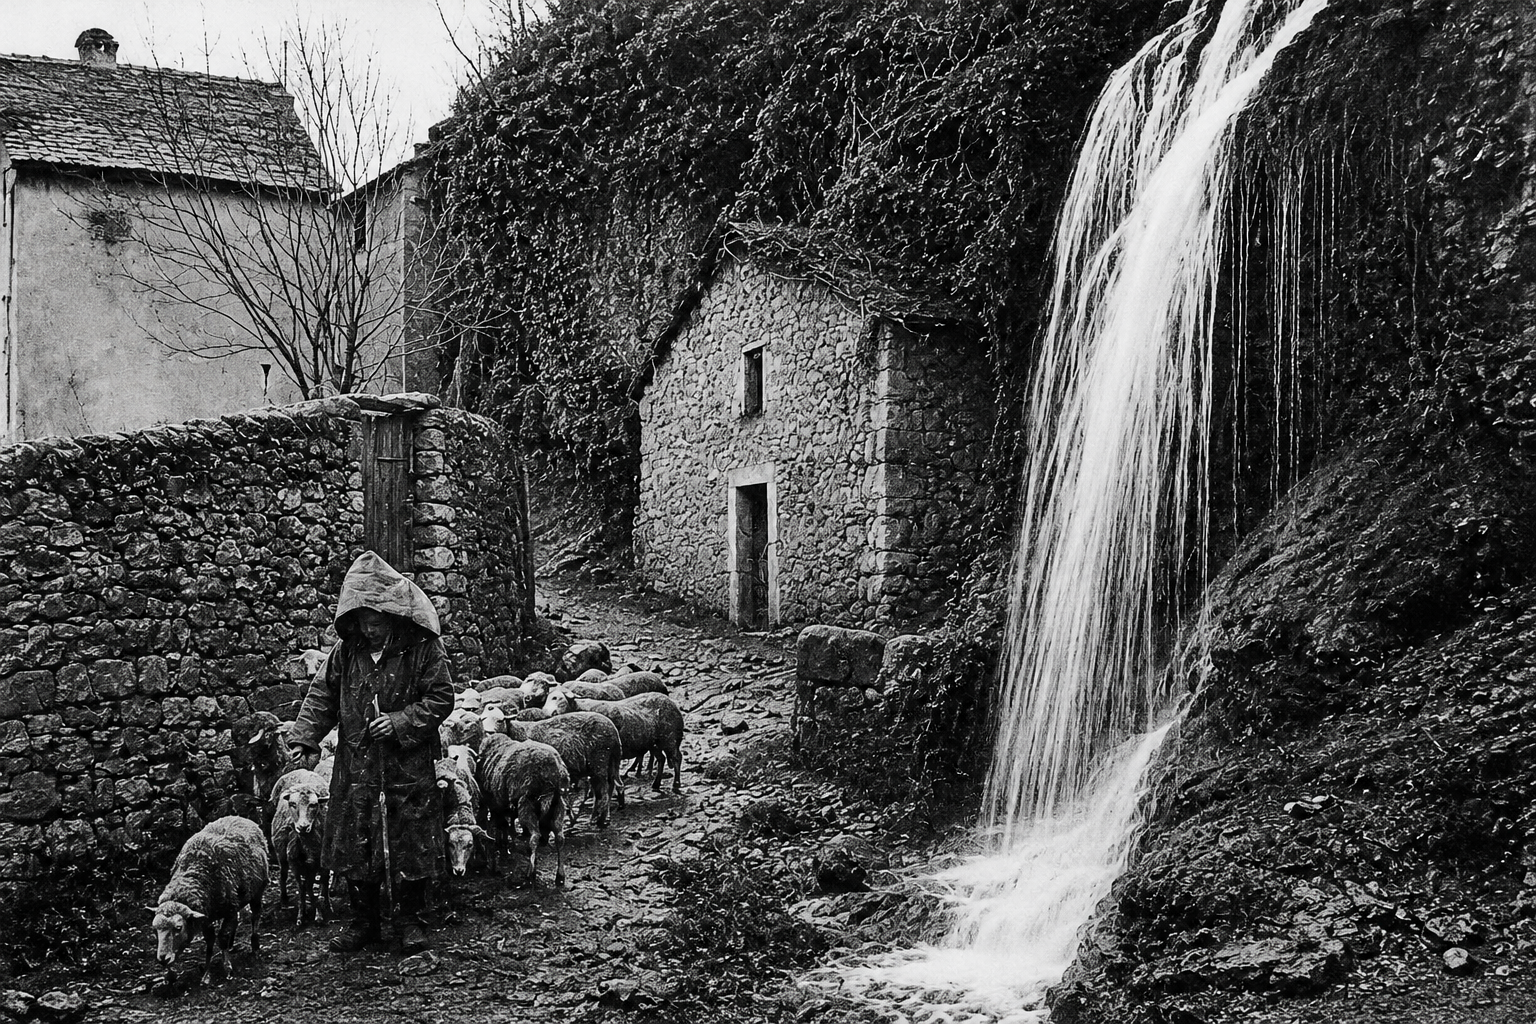
\includegraphics[width=\textwidth]{imgs/040.png}
\end{center}

\clearpage

\input{pages/019-entre-deux-guerres}
\clearpage

% Page 043 — page imprimée 39
% Contenu seul : le préambule, l'en-tête et la pagination sont gérés par meyrueis.tex

\sectiondate{Bonnes pages des souvenirs de Jean Gounelle (1902-1994)}{1933-1935}

\begin{center}
\vspace{0.4em}
\textbf{Pasteur de Meyrueis de 1932 à 1935}
\end{center}

Avec Meyrueis le jeune ménage pastoral que nous formions, Irène et moi, abordait un
pays plus civilisé que le Pompidou. Le territoire paroissial qui, désormais, allait nous
incomber comportait une petite ville et trois vallées.

Meyrueis constituait alors, comme aujourd’hui encore, un centre avec docteur,
dentiste, PTT, pharmacien, garage, Caisse d’Epargne, Banque, et beaucoup de
magasins etc. pourvu en outre de nombreux hôtels, dont certains luxueux. On sentait
la petite cité touristique, soignée, attirante, se suffisant à elle même, susceptible
d’accueillir une clientèle exigeante.

La population de ce bourg se rattachait, en grande partie, à l’Eglise Catholique. Les
protestants, majoritaires au 19\textsuperscript{e} siècle, ayant les premiers et assez massivement quitté
la ville, les Caussenards venaient combler les vides ainsi créés. L’école laïque ne
conservait qu’une influence secondaire par rapport à l’école libre, tenue par de jeunes
frères, instituteurs en soutane, très dynamiques et animés d’un grand zèle. De plus s’y
trouvait implantée une maison de « sœurs des pauvres » Ces femmes, d’un
dévouement sans borne, travaillaient dans ce milieu, appréciées de tous.
Notre ministère où la partie médicale avait tenu un si grand rôle au Pompidou, ne
pouvait qu’en être profondément modifié. Ce côté cependant, n’en fut pas pour
autant négligeable. !!

Notre action s’engagea surtout dans les trois vallées, entièrement protestantes elles,
celle de la Jonte, de la Brèze et du Bétuzon, trois ruisseaux dont les noms poétiques
chantaient comme le bruissement de leurs eaux. Ces trois vallées se rejoignaient à
l’endroit même où n’avait pu que surgir, dans la nuit des temps, un groupement
humain, protégé, cohérent et naturel.
Je ne vois pas d’autre explication à la naissance et à l’origine de Meyrueis.

Pour rester dans les considérations générales et m’en tenir à ce qui constituait ma
charge en ce lieu, disons que la paroisse protestante, dans les années 1930, avait un
double visage. Celui de l’hiver dans l’axe de ces trois vallées où se trouvaient nos
paysans, beaucoup plus à l’aise que ceux du Pompidou, à cause de leur lait de brebis
exploité par les caves de Roquefort. Celui de l’été. De Juin à Octobre, l’auditoire au
culte, nombreux et divers, se composait surtout de fidèles issus de grandes paroisses
citadines. Le Château d’Ayres, en particulier, dont le propriétaire faisait partie du
Conseil Presbytéral, constituait un pôle d’attraction exceptionnel.

Nos familles bourgeoises protestantes de Paris et d’ailleurs venaient volontiers y
passer l’été et revenaient ensuite. Elles animaient, nos « ventes », nos fêtes d’Eglise
organisaient au Temple de nombreuses rencontres et parfois de magnifiques concerts.
Le pasteur devait donc s’adapter à ce double aspect de l’Eglise locale, et ne pas
négliger les uns aux dépens des autres. Il convient également de se souvenir qu’en ces temps-là le tourisme constituait un luxe réservé à quelques privilégiés et que les
vacances étaient surtout le fait d’une élite et non pas généralisées comme aujourd’hui.
Les problèmes avaient donc peu de rapport avec ceux rencontrés au Pompidou, sauf
qu’il fallait, à travers un complexe différent en ces deux centres lozériens, faire
entendre le même message de paix, d’amour, de lumière et de justice: le message de
l’Evangile.[\ldots]

\subsection{Juillet 1932 : Installation à Meyrueis}

Ce mois de juillet fut, cette année là, particulièrement pluvieux. C’est sous les
parapluies et dans la boue que s’effectuèrent nos premiers contacts avec la
population. Notre adaptation ne fut certainement pas facilitée par la clémence du
temps ! J’avais peine à croire que le dépassement de la ligne de partage des eaux qui
séparait le Pompidou de Meyrueis pût amener de tels contrastes de climat. La
Cévenne elle même différait profondément. L’absence de châtaigniers ici était totale
(sauf dans les deux vallées schisteuses et granitiques du Bétuzon et de la Brèze, voire au dessus du
château d’Ayres). Tourné vers l’Atlantique, le paysage se montrait humide, plus
verdoyant, moins abrupt avec cependant, des entailles profondes à la séparation des
Causses, préfigurant déjà les Gorges du Tarn. Bref un changement plus accentué que
prévu.

Cette première impression plutôt fâcheuse fut compensée par notre prise de
possession d’un presbytère vraiment confortable pour l’époque.
Mon prédécesseur le pasteur Albert Chaudier, l’avait laissé en parfait état. Il avait
même voulu, en guise de bienvenue, que les pièces fussent retapissées à neuf pour
nous. Cela nous toucha beaucoup. Quel progrès sur ce que nous quittions ! Eau
courante, cheminées dans toutes les pièces au rez-de-chaussée et au premier,
harmonie dans la disposition de l’ensemble. La cuisine, la salle de séjour et le bureau
donnaient par plusieurs sorties sur un agréable jardin, hautement clôturé, que
remplissaient deux immenses poiriers chargés de fruits. Un conseiller presbytéral
facétieux, me disait « Il conviendrait d’appeler votre demeure « la villa des poires ».
Le moment n’était pas encore venu de posséder une salle de bains installée ni de
toilettes intérieures. Mais ces dernières se trouvaient à proximité et tout pouvait se
passer dans la plus normale discrétion. !

Très conscients de cette situation améliorée, quelle fut notre première préoccupation ?
Aussi inattendue que soit la réponse, la vérité m’oblige à la donner : mettre en route
un enfant.

[ La grossesse fut délicate et le premier-né vit le jour à la Maison de Santé de Nîmes. On l’appela
André, il devint pasteur... comme son père, puis professeur à la faculté de Théologie de Montpellier
écrivit de nombreux livres... ]

Mon ministère fut renouvelé par le bonheur de cette naissance... Je visitai d’arrache-
pied. J’organisai aussi parfaitement que possible mon enseignement auprès des
enfants et des jeunes, écoles du dimanche, du jeudi, catéchismes, Union Chrétienne.
Je montai une chorale et animai des réunions le soir. Je suppléai ainsi à l’absence
momentanée de collaboration de ma femme, absorbée, au début tout au moins, par
son bébé. Mais elle reprit assez vite sa place. Nous avions pu nous faire aider par la
fille d’un conseiller presbytéral, Jeanne Poujol (fille des Poujol, fermiers de la Fabrique) qui se mit à notre service et nous épaula avec beaucoup de dévouement. Les jours de
veillées ou de réunions, Irène pouvait m’accompagner. Au retour, dans la nuit, je
ramenai Jeanne chez elle.

Il y eut, au cours de notre séjour, ici et là, quelques soins médicaux à donner. Bien
plus tard, venant d’Afrique du Nord en vacances et de passage dans la région, tel ou
tel ancien paroissien de Meyrueis ou de Gatuzières nous disait : « Vous souvenez-
vous, Madame Gounelle vous avez soigné ma fille », « vous avez guéri la grand
mère », » « vous avez avant notre départ donné le landau d’André ce qui nous a
soulagés » « Quand ma mère, alitée depuis longtemps, souffrait de nombreuses
escarres, vous avez arrangé son lit et amélioré sa position en sorte que ses
souffrances furent considérablement allégées mais une heure plus tard elle
recommença à souffrir et me disais : Si notre dame était là ! »
Ce côté de notre mission restait bien réel. Mais au Pompidou, évidemment, sans
docteur et sans bonnes sœurs la trace s’était montrée bien plus profonde.
C’est ainsi que, sans éclat particulier, dans la fidélité aux petites choses, se déroula un
ministère paroissial normal, sans heurts et sans secousses, pendant trois ans.

\subsection{Notre concierge Monsieur Avesque (dit Lou Rascle)}

Un autre trait particulier du Meyrueis de 1930 c’est la personnalité de notre
concierge. Il s’appelait monsieur Avesque. Grand et original, fin parfois dans ses
réflexions, obstiné dans son comportement, vulgaire trop souvent dans son langage, il
avait le don d’imposer sa manière de faire, sans nuance. Très âgé, il avait dû, dans sa
jeunesse être un vrai colosse. Courbé par les ans, il restait encore très vigoureux.
Chaque semaine, il passait une journée entière, pour une rémunération dérisoire, à
nettoyer ce temple immense, briquer ses pavés disjoints, enlever la poussière de ses
bancs tous numérotés, garnir l’hiver les trois grands poêles, bien incapables d’ailleurs
de fournir une chaleur suffisante. Aussi chacun portait son chauffe-pied pour le
service du dimanche, qu’il avait préparé aussi bien que possible.

Après avoir allumé les feux ( il disait éclairé le feu ), le moment venu, il s’attaquait à
la lourde cloche, au son grave et profond, qui se répercutait au loin dans les vallées,
trois fois dans la matinée. Le dernier coup indiquait le début de l’office. Très souvent,
l’église catholique annonçait sa messe à la même heure. M. Avesque n’admettait pas
que nos « frères séparés » (ainsi les désignait-il) mettent leur cloche en branle tant
qu’il n’avait pas terminé. S’il avait commencé le premier, on devait respecter sa
priorité. Sinon il n’arrêtait pas de tirer sur sa corde. Cela aurait pu durer une demi-
heure, ou davantage, il ne cédait pas souvent, impuissant devant cette guerre des
cloches, j’ai été contraint de retarder « ma cérémonie » (sic) car il fallait bien, que le
silence se fit.

\subsection{Vie de l’église}

L’école du dimanche précédant le culte réunissait de nombreux élèves, pas toujours
très disciplinés. Je tenais beaucoup à ce qu’il y règne une certaine liberté et que cette
école ne ressemble pas, cet égard, à l’école de chaque jour. Nous avions plusieurs
groupes avant l’assemblée générale. Après le rassemblement, quand M. Avesque
s’apercevait qu’un garçon chahutait un peu trop à son gré, ne me trouvant pas assez
sévère, il faisait chauffer son tisonnier à blanc, puis, en pleine leçon il l’approchait, menaçant, de la figure du garnement, au risque de provoquer un accident. Les enfants
se tenaient tranquilles ; terrifiés par le concierge. Plusieurs, devenus vieux
aujourd’hui, en gardent le souvenir ! Ils me l’ont confirmé il y a peu de temps !
\emph{(je revois encore, en 1940, le Rascle nous poursuivant dans le temple avec son tisonnier, car nous le
faisions enrager ; chauffé à blanc ? bien sûr que non ! se souvient Paul Loupiac)}

Quant aux baptêmes, mariages et enterrements, il exigeait que les familles, après
s’être entretenues avec le pasteur, aillent le trouver, et surtout ne l’oublient pas sous
peine de ne pouvoir accéder au temple, qu’il estimait être un peu sa propriété
personnelle. En cas de négligence, il menaçait de prendre le large à l’heure de la
cérémonie, et de se rendre avec les clefs dans sa poche dans son champ le plus
éloigné. Cela arriva au moins une fois et n’amusa personne !!!

Irène tenait habituellement l’harmonium. Mais, avant et après la naissance d’André,
elle dut renoncer provisoirement à cette charge. Elle fut remplacée par une jeune fille
pleine de bonne volonté, mais qui ne pouvait accompagner les cantiques que d’une
main. L’instrument était bon, un harmonium de quatre jeux et demi, tout à fait adapté
à l’édifice. Un dimanche où je mettais au point avec un groupe de fidèles et
l’organiste, la partie musicale, Mr. Avesque s’approcha de nous et dit :
« \emph{Mademoiselle Agulhon, vous êtes beaucoup plus forte que le pasteur. Lui il a
besoin de deux mains pour jouer, vous, vous vous en tirez avec un doigt !} » On
pouvait considérer qu’il s’agissait d’une réflexion amusante dont on aurait dû
seulement sourire, mais cela déplut visiblement à l’organiste !

A cette période vivait à Meyrueis un pasteur à la retraite, originaire du pays, tout à
fait digne et remarquable. Il se nommait David Poujol\footnote{David Poujol était l’oncle de Marcel Poujol dit « Poujol d’Alger », rue saint blaise, décédé en 1994.}. Le concierge avait usé avec
lui ses fonds de culotte sur les bancs de l'école communale de Meyrueis. Ce pasteur
avait dirigé des églises importantes, Mazamet, Nîmes, La Haye et d’autres lieux.
Orateur incontestable, doué d’une puissante voix, on le sentait habitué aux nombreux
rassemblements. Il cultivait l’éloquence classique à laquelle il excellait. Un
dimanche, alors qu’il montait en chaire (où il me remplaçait, accompagné du
concierge qui le tutoyait depuis toujours, ce dernier lui dit devant moi : « \emph{Alors
David, c’est toi qui vas faire l’article aujourd’hui ?} » ce qui lui attira une verte
réplique, méritée, qui lui cloua le bec !
Je désire rendre hommage à ce pasteur distingué, disparu depuis longtemps, et qui
imposait le respect. Il finissait ses jours à Meyrueis où il vivait dans sa modeste
maison veuf et seul. Au gros de l’hiver il se rendait chez une de ses filles mais
revenait très vite. C’était un ramasseur de champignons. [\ldots]

Puisque je parle de David Poujol, comment ne pas mentionner le rayonnement de
deux autres pasteurs qui passaient, à cette époque leurs vacances d’été à Meyrueis.
Emile Guiraud de Paris et Louis Hubac de Castres. Ce dernier était le fils d’un paysan
que nous appréciions beaucoup, habitant la vallée de la Brèze, propriétaire de la
ferme de Conillergues près de Campis. Lorsqu’il prêchait, le temple se remplissait.
Sa prédication originale ( je me souviens d’un sermon sur « la main ») attirait, mais
n’était-il pas, surtout, un enfant du pays ?

Il passait régulièrement au presbytère, une ou deux fois par semaine, pour me
demander si j’étais libre. Il m’est arrivé assez souvent de l’accompagner. J’ai ainsi
pris contact, grâce à lui, avec une population catholique assez arriérée, de l’avis
même du docteur, mais qui s’est toujours montrée heureuse et même honorée d’être
visitée par un pasteur, dépourvu, de toute évidence, d’esprit de propagande ou de
prosélytisme.

A propos de ces traversées des Causses j’ai présenté à la mémoire un voyage en car
que j’y fis un jour, je ne sais plus pour quelle raison. Au départ de Meyrueis, au
dernier moment, un jeune curé vint s’asseoir à côté de moi, très exubérant et gentil
au possible, il engagea avec moi une conversation intéressante et animée. Au fur et à
mesure de l’entretien, une véritable sympathie s’établit entre nous deux. Quelle
agréable compagnie pour ce déplacement ! Puis, m’interrogeant plus directement, il
voulut savoir qui j’étais. Je n’avais aucune raison de le lui cacher : le pasteur de
Meyrueis. L’effet fut immédiat. Il me tourna carrément le dos et plus un mot ne sortit
de sa bouche. Quand il descendit , il ne me dit même pas au revoir !
Je n’ai jamais oublié cette attitude blessante, et il m’est arrivé, plus tard au cours de
réunions œcuméniques au Maroc, par exemple, avec d’autres curés, de raconter ce
petit incident pénible pour me réjouir qu’aujourd’hui, ce genre de comportement ne
serait ni possible ni concevable.

Même si des désaccords doctrinaux subsistent, au moins nous avons vis à vis les uns
des autres une attitude fraternelle grâce au Concile Vatican II et au pape Jean XXIII.

Enfin un mot sur les concerts. Il y en eut beaucoup au cours de notre séjour. Les plus
appréciés furent de deux sortes :

Ceux organisés avec le concours du célèbre violoncelliste de l’époque, d’origine
cévenole Jacques Serres. Il vient de mourir au moment où j’écris ces lignes. J’avais
béni, à Valleraugue son mariage avec la pianiste Ady Levastré. C’était vraiment du
grand art et le milieu estivant, très mélomane se trouvait à même de l’apprécier.
J’ajoute que le milieu paysan ne se montrait pas insensible au talent de cet artiste.

Je l’accompagnai à l’harmonium avec le souci évident de le mettre en valeur, mais en
m’efforçant quand même de dégager toutes les ressources de cet instrument, trop
décrié, de nos temples ou églises de montagne. Ensuite, de Meyrueis, nous étendîmes
notre audience à d’autres paroisses de la région, puis jusqu’à Pau, Millau, Montauban
et plus tard l’Afrique du nord

La seconde série de concerts se fit, en particulier, avec le concours d’une personne
qui faisait partie des vacanciers habituels, la Comtesse de Trémeuge. Cette femme
jeune, assez extraordinaire d’une grande beauté, avait reçu de la nature une voix
admirable. Elle n’appartenait pas à notre église, mais aimait fréquenter notre
presbytère. Elle admirait le dépouillement de la foi réformée. Devant cette artiste,
séduit par sa valeur et sa personne, je lui avais conseillé de lui permettre au moins du Bach du
Haendel ou du Franck. Je lui avais fait répéter, à la maison, des extraits de la Passion
selon St-Matthieu. Elle s’arrêta net et modestement, j’ajoute sagement, elle me
conseilla de lui permettre de chanter nos beaux cantiques, soigneusement
sélectionnés. Le succès fut total.

Quant au pasteur Guiraud, incomparable orateur, doué d’une voix plus distinguée que
forte, quel enchantement que d’entendre cet homme ! Je me souviens d’une prière de
lui, entendue à Meyrueis, qui commençait par cette invocation : « \emph{O Toi qui donnes,
Dieu de Noël, O Toi qui pardonnes, Dieu de Pâques, nous venons à Toi !} [\ldots]

Pendant deux ans, les circonstances locales s’y prêtant, je fis la classe de 6\textsuperscript{e} et de 5\textsuperscript{e} à
une jeune fille très douée, dont les parents, excellents paroissiens, ne voulaient pas se
séparer. Elle s’appelait Jeanine Fabre.
Je me fis donc professeur. Ma femme et moi prîmes en charge toutes les matières du
programme : français, latin, anglais, histoire, géographie, botanique géologie etc. La
suite de ces leçons elle fut admise avec félicitations dans un lycée de la capitale. Outre
la joie que l’on éprouve quand on a à faire à une enfant intelligente, cela apporta un
peu d’aisance à notre foyer qui en avait bien besoin. La contre-partie, un peu fâcheuse
c’est que toutes nos matinées furent prises. Autre conséquence : un bruit favorable se
répandit autour de ces leçons, et des vacanciers voulurent également que, au cours de
l’été, je fasse travailler leurs enfants. Je ne m’y suis pas refusé.

Janine Fabre, après y avoir fait ses études, fut nommée professeur de lettres au Lycée
Victor Duruy dans le 7\textsuperscript{e} Arrondissement.

\begin{itemize}
\item \emph{Plus tard elle épousa Francis Nougarède, ingénieur géologue. Ils eurent trois enfants,
Florence, Olivier et Pascal qui revenaient ensemble ou à tour de rôle au « Clair Logis »
leur maison de Meyrueis qui avait auparavant appartenu à la tante de Janine, le Dr. Juliette
Cabanel,
Francis fut emporté par une tumeur en 2004 et Janine le suivit un an plus tard.}
\end{itemize}

\emph{« Le Clair Logis » est passé désormais en d’autres mains.}

Nous avions aussi au mois de juillet et d’août étudiants en Théologie ou en Lettres
comme pensionnaires. Au nombre de 3 ou 4 chaque fois. Ils nous étaient envoyés par
l’Association Libérale de Strasbourg. Nous les faisions coucher dans deux vastes
chambres au premier. Toute la journée ils couraient dans les montagnes, visitaient la
région et, le soir venu, ils entonnaient des cantiques au presbytère. Cela tenait lieu de
culte de famille. Quel ne fut pas notre étonnement de constater que des
rassemblements assez importants de touristes se formaient autour de notre demeure
pour les écouter chaque jour ! Ces voix d’hommes étaient très belles et le sens musical
de ces jeunes strasbourgeois incontestable !

Comment ne pas mentionner nos rapports avec le Docteur Lapeyre et mes escapades
en sa compagnie sur les Causses. Dans une petite cité les rapports entre le pasteur et
Le médecin sont très importants, à tous égards. A Meyrueis, le docteur, catholique
pratiquant, préférait la compagnie du pasteur à celle du prêtre. Il l’avait déjà montré
avec un de mes prédécesseurs, M. Maurin.
Sa clientèle, en dehors du centre et des vallées, s’étendait sur les Causses, territoire
dont les habitants m’étaient inconnus, car je n’y avais aucun paroissien. Son rayon
d’action atteignait la Malène et Sainte Enimie, sur le Tarn, juste avant les Gorges
proprement dites. n’aimait pas rouler seul dans sa voiture, une belle conduite
intérieure Citroën confortable.


\subsection{Climat général en 1932 -- 1935}

De profonds changements se dessinèrent au cours de ces trois années. Les mutations
ne datent pas d’aujourd’hui seulement... la radio s’étendait partout et prenait une
grande place dans la vie de nos campagnes. Nous avions acquis un petit poste « Point
Bleu » bien insuffisant et modeste, mais nous l’écoutions tous les jours. Grâce à une
antenne tendue depuis le clocher du temple jusqu’au toit du presbytère, en l’absence
de moteurs et d’appareils ménagers, je captais les émissions avec une grande pureté.
C’était l’époque où les vedettes se nommaient Gaby Morlay, Sim Viva ou la
danseuse Mitsi, beautés lointaines et inconnues mais derrière le nom desquelles
j’imaginais la grâce féminine parisienne. L’époque également, hélas, des grands
scandales financiers, Stavisky et autres.

Puis ce fut le 6 Février 1934 et surtout le début des hurlements sinistres d’un inconnu
qui se nommait Adolf Hitler. Vraiment j’avais le sentiment que la relative tranquillité
que nous avions connue depuis l’armistice de 1919 était, bel et bien, en train de
disparaître.

Voilà un éclairage bien incomplet de ce temps de Meyrueis. Je pourrais développer.
Parler de Millau, de Florac, de nos veillées à Gatuzières ou à Cabrillac, de nos
campagnes « Christianisme Social », de nos représentations théâtrales avec les jeunes
etc Tout cela fut fort intéressant, remarquable même. Mais pourquoi le temps passé à
Meyrueis fut-il si court ?...

\emph{[... ( Jean Gounelle, comme plusieurs membres de sa famille, était attiré par l’Afrique du Nord :
l’énigme de ces pays évangélisés aux premiers siècles, leur essor, puis l’élimination à peu près totale
des églises chrétiennes par l’Islam du 8\textsuperscript{o} au 12\textsuperscript{o} siècle... Ne serait-ce pas le moment de s’y
réimplanter ? Oran n’avait plus de pasteur... Il fut nommé... et partit sans attendre... )....]}

Mais, cinquante ans plus tard, je conserve au fond de mon cœur, empreint d’une
certaine nostalgie, l’apport précieux que fut pour nous notre bref séjour à Meyrueis.
Et quand j’y retourne maintenant de Mandagout, (\emph{près du Vigan}) je perçois mieux, me
semble-t-il, les richesses et les bénédictions reçues dans cette humble cité ! Je m’en
souviens comme on se souvient avec émotion de ces périodes de préparation intense,
aussi bien intérieure que sur le terrain, où, loin des apparences et guidé par une main
invisible, se joue vraiment le destin d’un homme.

\clearpage

\input{pages/021-chantiers-jeunesse}
\clearpage

% Page 063 — page imprimée 60
% MEYRUEIS DE 1942 à 1944
% Notes prises par Marceline Causse de Pradines

\sectiondate{Meyrueis de 1942 à 1944}{1942-1944}

\begin{center}
\vspace{0.5em}
{\bfseries Notes prises par Marceline Causse de Pradines}
\end{center}

\medskip

\subsection{Après le combat d’Aire de Côte le 1\textsuperscript{er} Juillet 1943}

Un rescapé Marcel Chacon de Nimes arrive à Meyrueis chez le Pasteur Frank Robert qui lui
fait une fausse carte d’identité comme jardinier du Château d’Ayres, lieu où il a travaillé sans
descendre à Meyrueis.

\medskip

\noindent\textit{Quelques mois plus tôt (?) } le pasteur Robert rappelle avoir camouflé à Meyrueis un jeune
israélite Diamant (était-ce son nom de guerre ?), fils d’un bijoutier d’Anvers, qui s’est laissé
attraper par la gendarmerie. Qu’est-il devenu ?

Il en fut de même pour un autre juif, Hamburger, horloger à Meyrueis, qui fut saisi par deux
allemands et enfourné dans une auto.

\medskip

\subsection{Les jeunes des Chantiers de Jeunesse (groupement 19)}

Frank Robert voit à la poste 150 jeunes qui téléphonent à leurs familles qu’ils partent au STO
(Service du Travail Obligatoire) en Allemagne et les encourage à ne pas y aller. Il apprend
plus tard que ces 150 sont arrivés seulement 13 à Grenoble ; le train arrivé dans la plaine
languedocienne s’arrêtait : s’évadait qui voulait.

\medskip

\subsection{Note de Frank Robert, pasteur de Meyrueis en 1944}

Meyrueis avait un chef du ravitaillement comme chef lieu de canton désigné par Vichy
Mr. Arbousset.. Frank Robert apprend par ce chef qu’un camion chargé de fromages
descendra du Causse et sera dirigé sur Millau pour l’Allemagne. Frank Robert monte alerter le
maquis de l’Espérou qui arrive et oblige le conducteur du camion à monter à l’Espérou, ce
qu’il fit ; et le ravitaillement fut ensuite distribué au maquis et à Meyrueis.

\medskip

\subsection{Combat de la Parade (dimanche 28 Mai 1944, jour de Pentecôte)}

A Jontanels se trouvait Karl déserteur allemand et lieutenant, blessé, chef du groupe des
déserteurs allemands du maquis Bir Hakeim, transporté par M. Rolland de Meyrueis. Le Dr.
Bouisset l’a plâtré. Il fut ensuite caché sur les hauteurs, dans la nature, au dessus de Jontanels
et dans une grotte sur le chemin de Cabrillac et revint sur l’Espérou.

\medskip

Le maire de Gatuzières fit une carte d’identité pour Arjona du maquis Bir Hakeim afin qu’il
se rende auprès de Karl et qu’il recherche des blessés que Rolland est allé guérir dans la vallée
de la Jonte (\textit{Il s’agissait de Damiani et de Fages dit Fafa de Meyrueis.} ) Ils passèrent
plusieurs jours au moulin d’Ayres, soignés par le Dr. Juliette Cabanel et ravitaillés par Paul
Loupiac.

Et à partir de ce moment lundi 29 Mai, après l’inhumation des victimes de la Parade,
Meyrueis est \underline{surveillé}.

Le 6 Juin 1944 dès 5h du matin, 17 camions de 20 hommes en armes cernaient la ville. Mais
vers 9h00 ces troupes quittèrent rapidement Meyrueis. C’était le jour du débarquement. Sans
le débarquement que serait devenu Meyrueis ?

\begin{quote}
\textit{(en partant par la route de Florac ils s’arrêtèrent devant le moulin d’Ayres et nous les vîmes
descendre pour une pause « pipi », Damiani, Fafa et moi. Quelle peur rétrospective !)}
\end{quote}

\medskip

\subsection{À Jerusalem}

\medskip

Une avenue partant vers le désert est plantée d’arbres. Les Israéliens veulent inscrire sur les
troncs les noms de Français qui ont protégé les Juifs entre 40 et 45 en Europe.

\medskip

Il est indiqué par M. Frank Robert de Nimes ancien pasteur de Meyruies, de 41 à 45 des
noms de Meyrueisiens :

Les Dr. Bouisset et J. Cabanel, M. Rolland transporteur

Mme. Roussel du Château d’Ayres, château qui a été un centre de camouflage de première
grandeur. Propriétaire, avec sa fille Ginette Teissier du Cros et son mari Jean

M. Harrisson frère de Mme. Roussel, chef de réseau,. Des personnes en danger sont restées
plusieurs années au Château.

Des habitants des vallées et de Jontanels.

M. Cahen Salvador président de chambre au Conseil d’Etat.

M. Jacques Pfeiffer avocat à Paris.

\medskip

Notes prises à la suite d’une conversation entre Frank Robert et Marceline Causse de
Pradines. Non daté…

\medskip

\textit{Les notes en italique ont été rajoutées pour la compréhension du texte par Paul Loupiac\\
Le 5 Septembre 2002 au Moulin d’Ayres.}



\clearpage

% Page 065 — page imprimée 62
% Anecdotes, Témoignages, Souvenirs…


\sectiondate{Anecdotes, Témoignages, Souvenirs…}{}


\medskip

\noindent{\bfseries EVA VERDIER} mère de Madeleine qui avait épousé Emilien Martin (originaire de
Rousses à 3km du Villaret dans la vallée du Bétuzon) raconte, à 104 ans, en 1986, à la
Bragousette où elle passa ses dernières années chez sa fille :

\medskip

\subsection{La soie}

\begin{quote}
\textit{« Quand j’étais jeune j’habitais aux Salides, un petit hameau sur la pente sous le col Salidès.
Les mûriers étaient nombreux dans la région et on élevait des vers à soie dans beaucoup de
fermes. Les cocons étaient vendus à St. André de Valborgne, et je faisais éclore quelques
onces de « graine ». Dès que j’avais 5kg de cocons je les portais à la filature à Saint André. »}
\end{quote}

\begin{quote}
\textit{« La Fabrique » à Meyrueis était alors une grande magnanerie, puis elle fut transformée en
filature. »}
\end{quote}

\medskip

\subsection{Un assassinat en 1826}

Celui de Monsieur de Fenouillet, Baron des Fons, (Les Fons est une grosse propriété à
quelques km. de Cabrillac sur la route de Saint André de Valborgne). C’est une histoire que
lui avait racontée son grand père :

\begin{quote}
\textit{« Monsieur de Fenouillet, propriétaire terrien vivant du revenu de ses terres cultivées par
des fermiers faisait confectionner par sa lingère habitant aux Salides (hameau en contrebas
du col Salidès) des sacs d’étoffe dans les quels il serrait les rouleaux d’écus qu’il amassait. Il
les cachait dans une pièce spéciale du château des Fons (était-ce son bureau ou sa cave, je ne
sais).}
\end{quote}

\begin{quote}
\textit{Trois jeunes gens des Salides décidèrent de le dévaliser. L’un d’eux, courtisant la lingère,
manœuvre habilement pour localiser le trésor, lui demandant d’abord de soustraire elle
même quelques sachets et se heurtant à un refus finit, après lui avoir demandé quel est son
travail principal, à quoi étaient destinés les sacs qu’elle cousait, comment et où ils étaient
rangés, à obtenir une nuit un rendez vous amoureux. Il la prie de laisser le soir une porte du
château ouverte.}
\end{quote}

\begin{quote}
\textit{Il pénétra alors la nuit avec ses deux acolytes et ils arrivèrent à la cachette, lorsque le baron
réveillé en sursaut par un bruit insolite se leva et leur barra la route. Pris de panique les trois
voleurs lui tranchèrent la gorge. Ils furent rapidement identifiés et condamnés à être
décapités.}
\end{quote}

\begin{quote}
\textit{La guillotine fut installée au Pompidou. Un jeune berger des Salides décida d’assister à
l’exécution pour « voir tomber les têtes ». Ce fut si horrible qu’il en perdit la raison. »}
\end{quote}

% Page 066 — page imprimée 63
% Suite de « Anecdotes, Témoignages, Souvenirs… »

Voilà donc ce récit conservé dans une famille, par la tradition orale. En fait il semble que si
cet assassinat a bien eu lieu, les pièces officielles, conservées à l’occasion du procès des
assassins les détails furent tout autres.

M. Maurice Abric de Fernouillet fut bien assassiné par trois hommes, le 16 janvier 1826 mais
au Château de l’Hom, une autre de ses propriétés, au Follaquier, hameau près de la route de
Saint André de Valborgne à quelques km des Salides et non pas aux Fons.
Sans doute y eut-il vol mais M. de Fenouillet, noble de fraîche date faisait preuve
d’arrogance, humiliant ses fermiers, corrigeant lui-même à coups de bâton deux enfants de 10
ans ! fils de son fermier, qui avaient dérobé quelques une de ses poires… n’hésitant pas à
couper les oreilles de chèvres qui avaient mangé ses châtaignes ou écorcé de jeunes
châtaigniers :

\begin{quote}
\textit{« …ce type là, raconte un habitant de Bassurel dans les années 1980, il aimait pas les gens.
Et alors les gens faisaient sortir leurs chèvres, comme ça. Et quand il trouvait des chèvres, il
leur coupait les oreilles ! Et quand ils ont vu ça, un jour ils l’ont tué, les voisins. Et je crois
qu’il est enterré là bas à l’Hom… Oh c’était une sale bête ! Il pouvait pas voir ses voisins,
quoi. »}
\end{quote}

Les trois assassins furent bel et bien condamnés à mort et guillotinés sur la place du
Pompidou le 7 mars 1827.

Cette triste histoire a tout de même causé la mort de quatre personnes, semé la désolation dans
plusieurs familles et laissé une dizaine d’orphelins dont certains n’ont pas connu leur père.

\begin{flushright}
Almanach de la Vallée Borgne 2006
\end{flushright}

\clearpage

\input{pages/024-trois-vallées}
\clearpage

\input{pages/025-figures-locales}
\clearpage

% ------------------------------------------------------------
% Page 94 bis
% ------------------------------------------------------------

\begin{tikzpicture}[remember picture,overlay]
    \node[
        anchor=south west,
        inner sep=0pt,
        opacity=0.60
    ] at (current page.south west) {%
        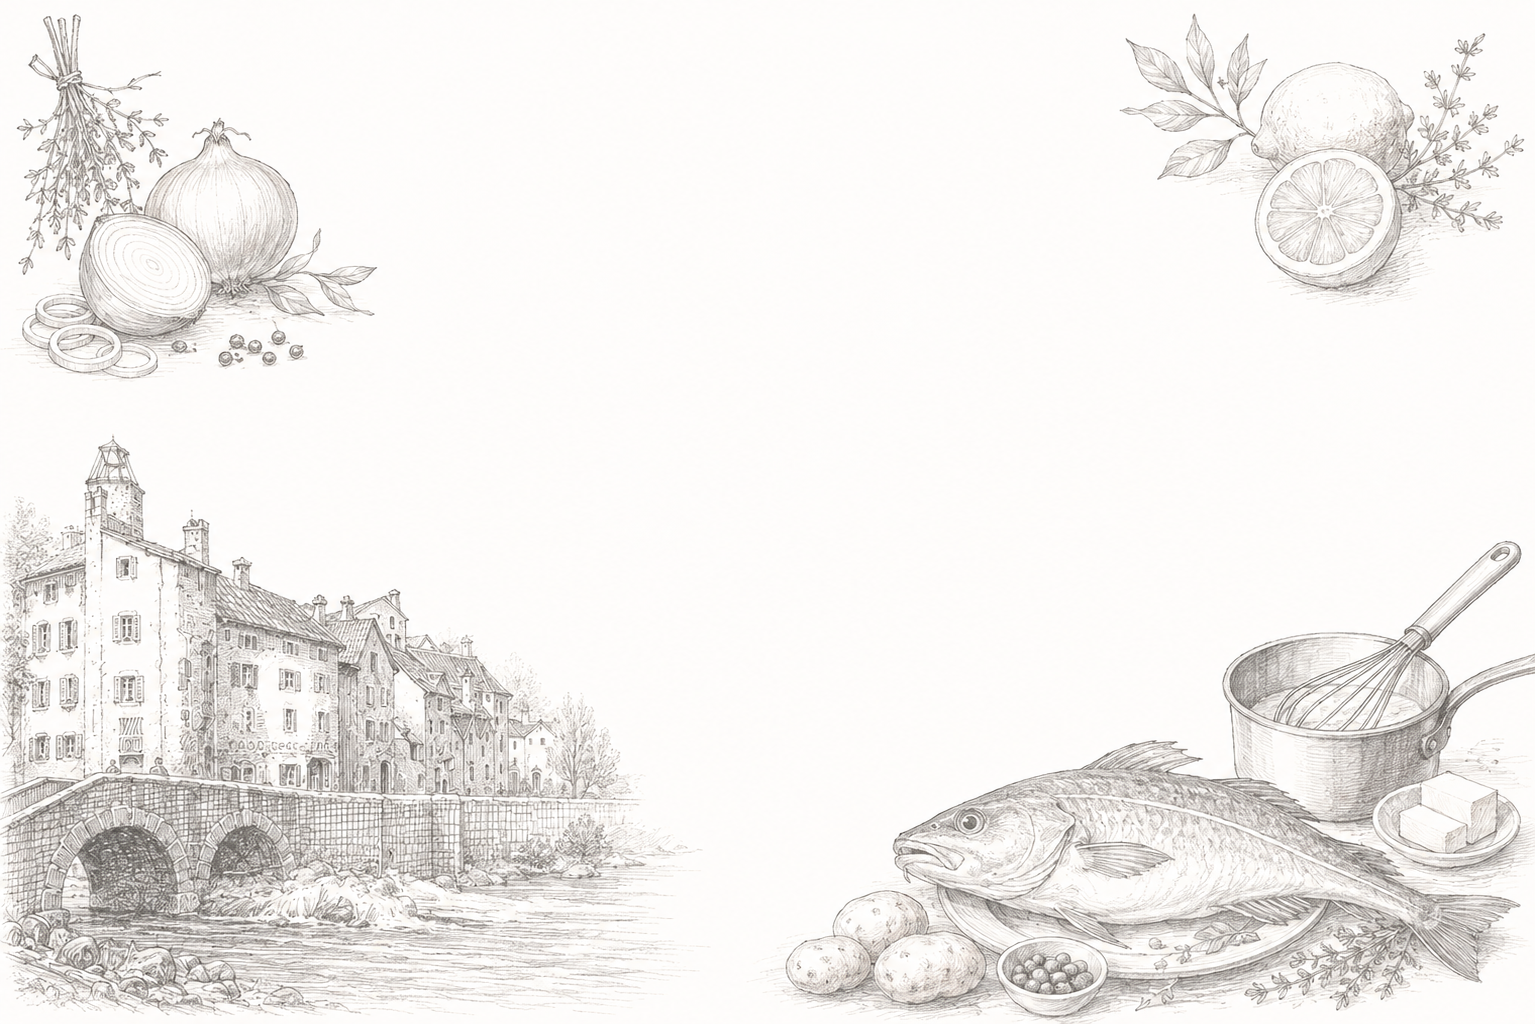
\includegraphics[
            width=\paperwidth,
            height=\paperheight
        ]{imgs/101}%
    };
\end{tikzpicture}

\sectiondate{Recette de la Morue à la Sauce Blanche}{}

{\fontspec{Comic Sans MS}
\large

\vspace{25mm}

Faire dessaler la morue, un ou deux jours à l’eau froide en renouvelant l’eau
régulièrement.

La mettre à cuire dans de l’eau froide avec des rondelles de citrons, des
tranches d’oignons, thym, laurier, poivre et un morceau de beurre.\\

Quand la morue est cuite la retirer et la tenir au chaud, faire cuire les pommes
de terre avec la même eau sans les éplucher auparavant.\\

Dresser le poisson sur un plat, les pommes de terre épluchées une fois cuites,
autour.\\

\textbf{Servir avec une sauce blanche}

Mettre dans une casserole 30 g de beurre frais, laisser fondre à blanc, ajouter
deux cuillerées de farine fine ; faire cuire quelques minutes à feu doux, en
remuant avec un fouet sans laisser prendre couleur. Y verser doucement de
l’eau bouillante, toujours en remuant avec le fouet pour éviter les grumeaux.\\

Saler, poivrer, laisser faire un bouillon et y incorporer, par petits morceaux,
30 nouveaux gr. de beurre ou un pot de crème.\\

Ne plus laisser cuire pour conserver à la crème son goût de beurre frais.

Si on en trouve à l’épicerie du coin, ajouter des câpres avant de servir.

Terminer par une liaison à l’œuf et un filet de jus de citron.}

\begin{center}
Quel délice ! Bon appétit !
\end{center}

\begin{flushright}
Marianne Loupiac\\
Juin 2006
\end{flushright}

\clearpage

\input{pages/027-épilogue}
\clearpage

\input{pages/028-quatrième-de-couverture}
\clearpage

\end{document}
